%%%%%%%%%%%%%%%%%%%%%%%%% 
% Dokumentinformationen %
%%%%%%%%%%%%%%%%%%%%%%%%%
\newcommand{\titleinfo}{Statistical Digital Signal Processing And Modeling}
\newcommand{\authorinfo}{L. Schmid, R. Koller, Ch. Schlittler, S. Eicher, H.Diethelm} % Do not remove any names! Initial authors stay first.
\newcommand{\versioninfo}{FS2014}

%%%%%%%%%%%%%%%%%%%%%%%%%%%%%%%%%%%%%%%%%%%%%
% Standard projektübergreifender Header für
% - Makros 
% - Farben
% - Mathematische Operatoren 
%
% DORT NUR ERGÄNZEN, NICHTS LÖSCHEN
%%%%%%%%%%%%%%%%%%%%%%%%%%%%%%%%%%%%%%%%%%%%%  
% Genereller Header
\documentclass[10pt,twoside,a4paper,fleqn]{article}
\usepackage[utf8]{inputenc}
\usepackage[left=1cm,right=1cm,top=1cm,bottom=1cm,includeheadfoot]{geometry}
\usepackage[ngerman]{babel,varioref}


% Pakete
\usepackage{amssymb}
\usepackage{amsmath}
\usepackage{fancybox}
\usepackage{bm}       % Bold Math
\usepackage{graphicx}
\usepackage{color}
\usepackage{lastpage}
\usepackage{wrapfig}
\usepackage{fancyhdr}
\usepackage{hyperref}
%\usepackage{verbatim}
%\usepackage{floatflt}
\usepackage{multirow} % zellen in tabellen verbinden
\usepackage{multicol} 

%\usepackage{arydshln}
\usepackage{ucs}
\usepackage{pdflscape} % landscape
%\usepackage{slashbox} % getrennte zelle in tabelle
%\usepackage{array} % anordnung in tabellen
%Show pdf in 100 zomm factor!
\usepackage{hyperref}
\hypersetup{pdfstartview={XYZ null null 1.00}}

%%%%%%%%%%%%%%%%%%%%
% Generelle Makros %
%%%%%%%%%%%%%%%%%%%%
\newcommand{\skript}[1]{$_{\textcolor{red}{\mbox{\small{Skript S. #1}}}}$}
\newcommand{\sachs}[1]{$_{\textcolor{blue}{\mbox{\small{Sachs S. #1}}}}$}
\newcommand{\formelbuch}[1]{$_{\textcolor{red}{\mbox{\small{S#1}}}}$}
\newcommand{\hayes}[1]{$_{\textcolor{red}{\mbox{\small{Hayes p #1}}}}$}
\newcommand{\verweis}[2]{ {\small (siehe auch \ref{#1}, #2 (S. \pageref{#1}))}}
\newcommand{\subsubadd}[1]{\textcolor{black}{\mbox{#1}}}
\newenvironment{liste}[0]{\begin{list}{$\bullet$}{\setlength{\itemsep}{0cm}\setlength{\parsep}{0cm} \setlength{\topsep}{0cm}}}{\end{list}}
    
\newcommand{\logd}[0]{\log_{10}}
\newcommand{\subsubsubsection}[1]{\textbf{#1}}
\newcommand{\matlab}[1]{\footnotesize{(Matlab: \texttt{#1})}\normalsize{}}

\newenvironment{aufzaehlung}[0]{\begin{enumerate}{\setlength{\itemsep}{0cm}\setlength{\parsep}{0cm}\setlength{\topsep}{0cm}}} {\end{enumerate}}

\newcommand{\abbHeight}[3]{
	\begin{center}
		\includegraphics[height=#2]{./bilder/#1} \\
		#3
    \end{center}
}

%\newcommand{\skriptsection}[2]{\section{#1 {\tiny Skript S. #2}}}
%\newcommand{\skriptsubsection}[2]{\subsection{#1 {\tiny Skript S. #2}}}
%\newcommand{\skriptsubsubsection}[2]{\subsubsection{#1 {\tiny Skript S. #2}}}
%\renewcommand{\skriptsection}[2]{\section{#1 {\tiny Schaum S. #2}}}
%\renewcommand{\skriptsubsection}[2]{\subsection{#1 {\tiny Schaum S. #2}}}
%\renewcommand{\skriptsubsubsection}[2]{\subsubsection{#1 {\tiny Schaum S. #2}}}
\newcommand{\skriptsection}[2]{\section{#1 \formelbuch{#2}}}
\newcommand{\skriptsubsection}[2]{\subsection{#1 \formelbuch{#2}}}
\newcommand{\skriptsubsubsection}[2]{\subsubsection{#1 \formelbuch{#2}}}

%%%%%%%%%%
% Farben %
%%%%%%%%%%
\definecolor{black}{rgb}{0,0,0}
\definecolor{red}{rgb}{1,0,0}
\definecolor{white}{rgb}{1,1,1}
\definecolor{grey}{rgb}{0.8,0.8,0.8}

%%%%%%%%%%%%%%%%%%%%%%%%%%%%
% Mathematische Operatoren %
%%%%%%%%%%%%%%%%%%%%%%%%%%%%
\DeclareMathOperator{\sinc}{sinc}
\DeclareMathOperator{\sgn}{sgn}
\DeclareMathOperator{\Real}{Re}
\DeclareMathOperator{\Imag}{Im}



% Fouriertransformationen
\unitlength1cm
\newcommand{\FT}
{
\begin{picture}(1,0.5)
\put(0.2,0.1){\circle{0.14}}\put(0.27,0.1){\line(1,0){0.5}}\put(0.77,0.1){\circle*{0.14}}
\end{picture}
}


\newcommand{\IFT}
{
\begin{picture}(1,0.5)
\put(0.2,0.1){\circle*{0.14}}\put(0.27,0.1){\line(1,0){0.45}}\put(0.77,0.1){\circle{0.14}}
\end{picture}
}
\newcommand{\jw}{j\omega}

\newcommand{\numbercircled}[1]{\textcircled{\raisebox{-1pt}{#1}}}

\newcommand{\DFT}
{
%\overset{DFT}{
	\begin{picture}(1,0.2)
	\put(0.2,0.1){\circle{0.14}}{\put(0.27,0.1){\line(1,0){0.5}}}\put(0.77,0.1){\circle*{0.14}}
	\end{picture}
%}
}

\newcommand{\IDFT}
{
%\overset{IDFT}{
    \begin{picture}(1,0.2)
	\put(0.2,0.1){\circle*{0.14}}\put(0.27,0.1){\line(1,0){0.45}}\put(0.77,0.1){\circle{0.14}}
	\end{picture}
%}
}



%%%%%%%%%%%%%%%%%%%%%%%%%%%%
% Allgemeine Einstellungen %
%%%%%%%%%%%%%%%%%%%%%%%%%%%%
%pdf info
\hypersetup{pdfauthor={\authorinfo},pdftitle={\titleinfo},colorlinks=false}
\author{\authorinfo}
\title{\titleinfo}

%Kopf- und Fusszeile
\pagestyle{fancy}
\fancyhf{}
%Linien oben und unten
\renewcommand{\headrulewidth}{0.5pt} 
\renewcommand{\footrulewidth}{0.5pt}


\fancyhead[L]{\titleinfo{ }- Summary}
%Kopfzeile rechts bzw. aussen
\fancyhead[R]{\today{ }- Page \thepage/\pageref{LastPage}}
\fancyfoot[C]{\copyright{ }\authorinfo}

% Einr�cken verhindern versuchen
\setlength{\parindent}{0pt}



\raggedbottom
% Möglichst keine Ergänzungen hier, sondern in header.tex
\begin{document} 
 
%%%%%%%%%%%%%%%%%%%%%%%%%%%%%%%%%%%%%%%%%%%%%%%%%%%%%%%%%%%%%%%%%%%%%%%%%%%%%%%%%%%%%%%%%%%%%%%
%%%%%%%%%%%%%%%%%%%%%%%%%%%%%%%%%%%%%%%%%%%%%%%%%%%%%%%%%%%%%%%%%%%%%%%%%%%%%%%%%%%%%%%%%%%%%%%

% Diskrete Fourier Transformation
\begin{landscape}

\begin{minipage}{7cm}
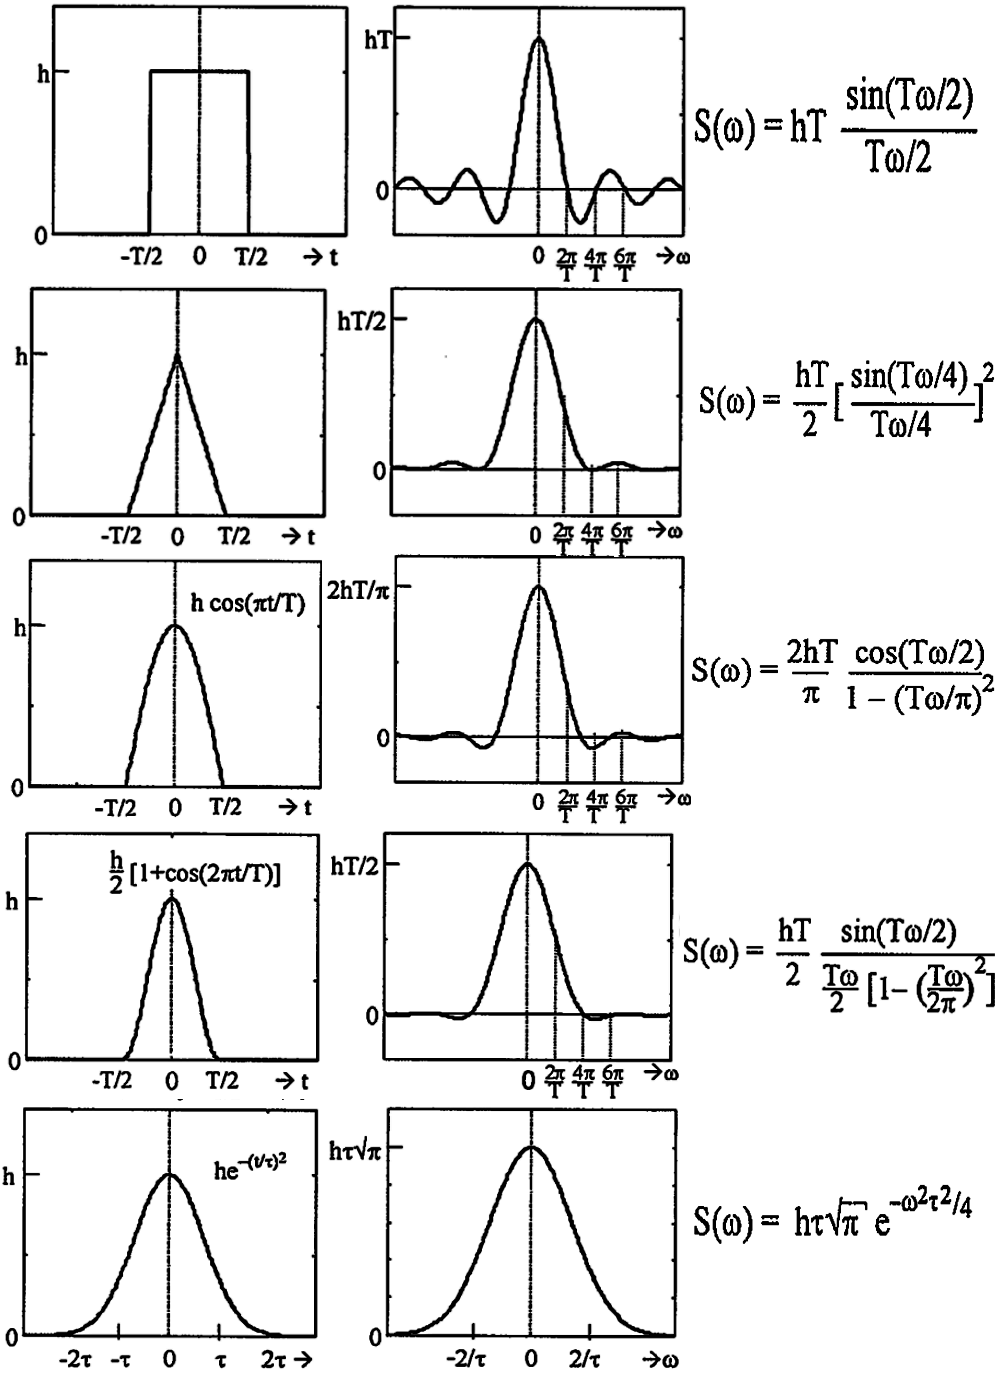
\includegraphics[width=\textwidth,trim= 0cm 0cm 0cm 0cm]{bilder/Transformationen/Fourier-Trafo.png}

\end{minipage}
\begin{minipage}{8.25cm}
	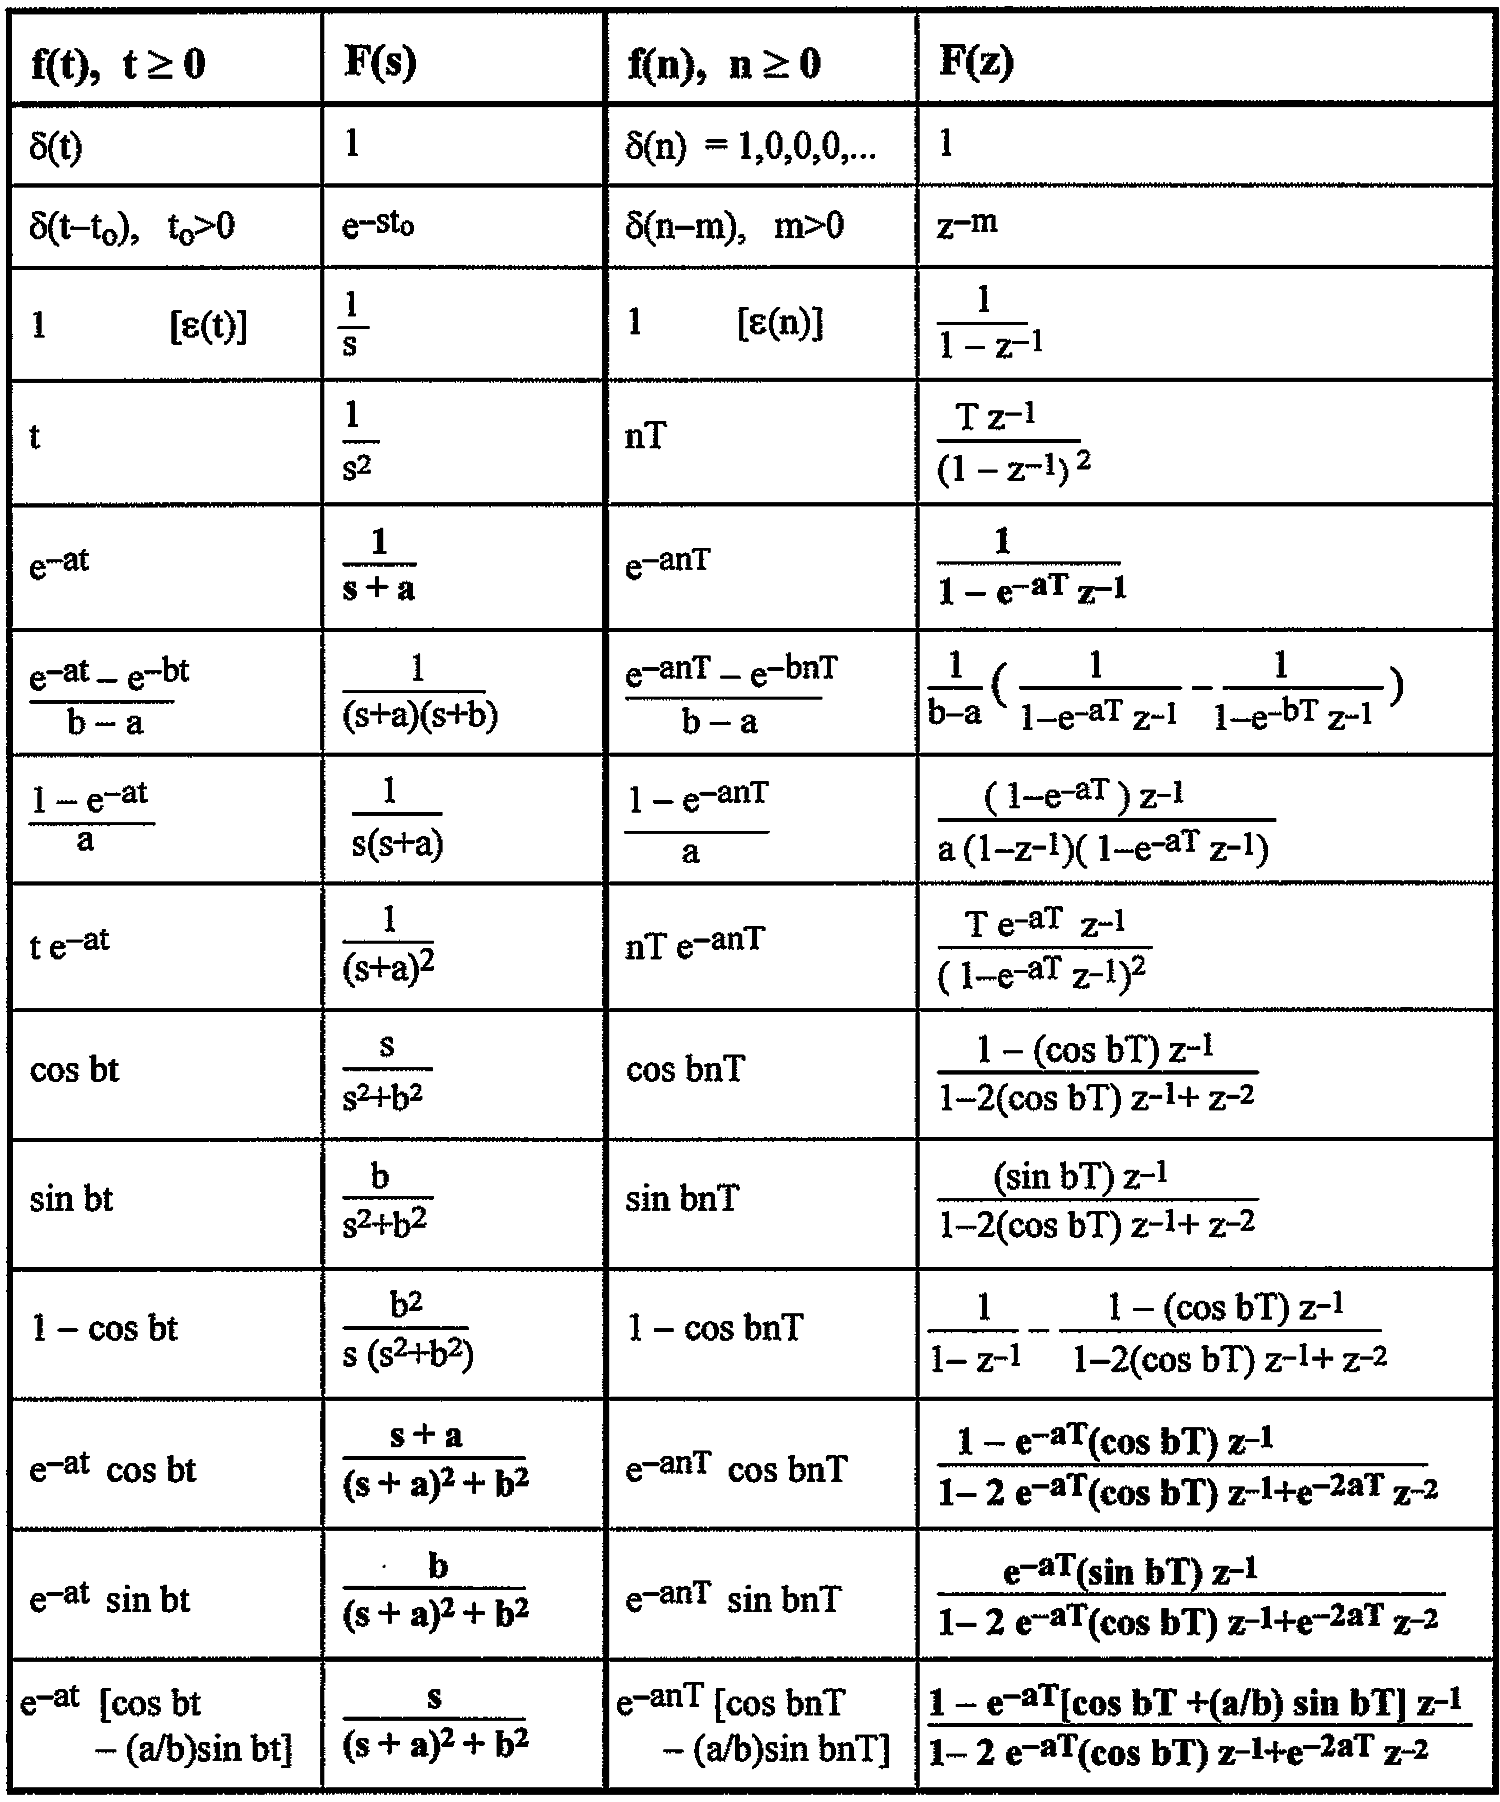
\includegraphics[width=\textwidth,trim= 0cm 0.3cm 0cm 0.45cm]{bilder/Transformationen/Z-Lexikon.png}
	\end{minipage}
	\begin{minipage}{10cm}
	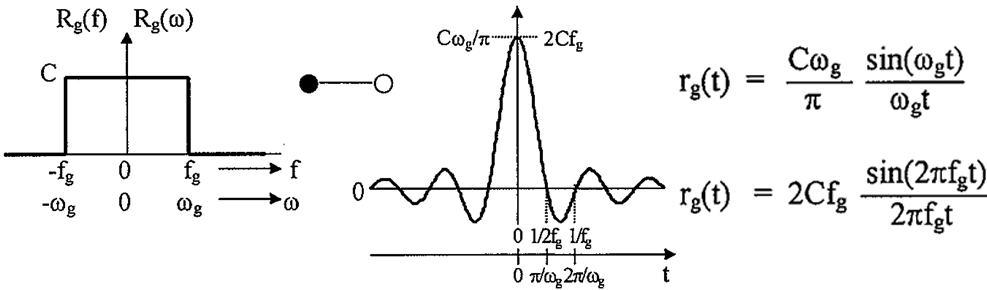
\includegraphics[width=\textwidth,trim= 0cm 0cm 0cm 0cm]{bilder/Transformationen/Rechteck-Sinc.png}
	\textbf{Matrizeninversion}\\
	$A^{-1} = \begin{pmatrix}
	a & b \\ c & d \\
	\end{pmatrix}^{-1} =
	\frac{1}{\det(A)} \begin{pmatrix}
	d & -b \\ -c & a \\
	\end{pmatrix}  =
	\frac{1}{ad-bc} \begin{pmatrix}
	d & -b \\ -c & a \\
	\end{pmatrix}\quad$\\
	$A^{-1} = \begin{pmatrix}
	a & b & c\\ d & e & f \\ g & h & i \\
	\end{pmatrix}^{-1} =
	\frac{1}{\det(A)} \begin{pmatrix}
	ei - fh & ch - bi & bf - ce \\
	fg - di & ai - cg & cd - af \\
	dh - eg & bg - ah & ae - bd
	\end{pmatrix}$\\
	\begin{minipage}{4cm}
		\textbf{Trigonometrie} \\
		$e^{j\varphi}=\cos(\varphi)+ j \cdot \sin(\varphi) $
		$e^{-j\varphi}=\cos(\varphi)- j \cdot \sin(\varphi) $
		$\cos(x) = \frac{e^{jx} + e^{-jx}}{2}$\\
		$\sin(x) = \frac{e^{jx} - e^{-jx}}{2j}$\\
		$\cos^2(x) = \frac12 + \frac{\cos(2x)}{2}$\\
		$\sin^2(x) = \frac12 - \frac{\cos(2x)}{2}$\\
		$\sin(2x)=2\sin(x)\cdot\cos(x)$\\
		$\sin^2(x)+\cos^2(x)=1$
	\end{minipage}
	\begin{minipage}{5cm}
		\textbf{Determinanten} \\
		\footnotesize
		$\det \begin{pmatrix} a & b \\ c & d\\ \end{pmatrix} =
		a d - b c \quad$\\
		$\det \begin{pmatrix} 
		a & b & c \\
		d & e & f \\
		g & h & i  \end{pmatrix}
		= a e i + b f g + c g h \\
		\text{\hspace{2.5cm}} -c e g - f h a - i b d$		\normalsize
	\end{minipage}
\end{minipage}

%\section{Fourier Transformation}
\begin{minipage}{0.85\linewidth}
%\subsubsection{Eigenschaften von Fourier- und Z-Transformation}
\footnotesize 
\renewcommand{\arraystretch}{1.1}
\begin{tabular}{|p{4.3cm}||p{1.8cm}|p{1.8cm}||p{2.2cm}|p{2.4cm}||p{1.9cm}|p{2.6cm}|}
\hline
\textbf{Bezeichnung}
  & \multicolumn{2}{|c||}{\textbf{Zeitbereich}}
  & \multicolumn{2}{|c||}{\textbf{Kontinuierlicher Frequenzbereich}}
  & \multicolumn{2}{|c|}{\textbf{Diskreter Frequenzbereich}} \\
  & \textbf{kontinuierlich}
  & \textbf{diskret}
  & \textbf{Fourier-Integral} 
  & \textbf{Laplace}
  & \textbf{Diskrete FT} 
  & \textbf{Z-Transformation} \\
\hline
\hline
  Linearität 
  & $\alpha\cdot f(t) + \beta\cdot g(t)$
  & $\alpha\cdot f(n) + \beta\cdot g(n)$
  & $\alpha\cdot F(\omega) + \beta\cdot G(\omega)$
  & $\alpha\cdot F(s) + \beta\cdot G(s)$
  & $\alpha\cdot F(n) + \beta\cdot G(n)$
  & $\alpha\cdot F(z) + \beta\cdot G(z)$\\
\hline
  "Ahnlichkeit / Zeitskalierung bzw. Spiegelung an Y-Achse
  &	$f(\alpha t)$ 
  & $f(-n)$
  & $\frac{1}{|\alpha|}F \left (\frac{\omega}{\alpha} \right)$
  & $\frac{1}{\alpha}F \left (\frac{s}{\alpha} \right )$ 
  & $F(-n)$
  & $F(z^{-1})$\\
%\hline
  %D�mpfung
  %& -
  %& $e^{dn} f(n)$
  %& -
  %& - 
  %& -
  %& $F(z e^{d})$ \\
\hline
  Verschiebung im Zeitbereich 
  & $f(t\pm t_0)$ 
  & $f(n \pm n_0)$
  & $e^{\pm j\omega t_0} F(\omega)$
  & $F(s)e^{\pm t_0 s}$ 
  & $e^{\pm j\frac{n}{N}2 \pi n_0} F(n)$
  & $z^{\pm n_0} F(z)$\\
\hline
  Verschiebung im Frequenzbereich 
  & $f(t)e^{\mp\alpha t}$ 
  & $f(n) e^{\mp j \frac{n}{N} 2 \pi n_0}$
  & $F(\omega\pm \alpha)$
  & $F(s\pm\alpha)$ 
  & $F(n \pm n_0)$
  & $F(z \pm n_0)$\\
\hline
  Faltung im Zeitbereich 
  &	$f(t) \ast g(t)$
  & $f(n) \ast g(n)$
  & $F(\omega) \cdot G(\omega)$
  & $F(s) \cdot G(s)$
  & $F(n) \cdot G(n)$ 
  & $F(z) \cdot G(z)$ \\
\hline
  Faltung im Frequenzbereich 
  &	$f(t) \cdot g(t)$
  & $f(n) \cdot g(n)$
  & $\frac{1}{2\pi} F(\omega) \ast G(\omega)$
  & $\frac{1}{2\pi} F(s) \ast G(s)$ 
  & $\frac{1}{N} F(n) \ast G(n)$
  & $\frac{1}{N} F(z) \ast G(z)$\\
\hline
  Ableitungen im Zeitbereich bzw. Differenzenbildung 
  & $\frac{\partial^n f(t)}{\partial t^n}$ 
  & $\Delta^k f(n)$
  & $(j\omega)^n F(\omega)$
  & $s^nF(s)-s^{n-1}f(0+)-s^{n-2}\frac{\partial f(0+)}{\partial t}-\ldots
 			-s^0\frac{\partial^{n-1} f(0+)}{\partial t^{n-1}}$
  & 
  & $(1-z^{-1})^k F(z)$ \\
\hline
  Ableitung im Frequenzbereich
  & $(-t)^k\cdot f(t)$ 
  & $n f(n)$ 
  & $j^k \frac{-\partial^k F(\omega)}{\partial \omega^k}$
  & $\frac{\partial^k F(s)}{\partial s^k}$
  & 
  & $-z \frac{\partial F(z)}{\partial z}$ \\
\hline 			
  Integration bzw. Summierung
  & $\int\limits_{-\infty}^t f(\tau)d\tau$ 
  & $\sum\limits_{n=0}^{k} f(n)$
  & $\frac{F(\omega)}{j\omega}+F(0)\pi\delta(\omega)$
  & $\frac{F(s)}{s}$
  & 
  & $\frac{1}{1-z^{-1}} F(z)$ \\
\hline
  Anfangswert 
  & $\lim\limits_{t\rightarrow 0} f(t)$ 
  & $f(0)$
  & 
  & $\lim\limits_{s\rightarrow \infty} sF(s)$ 
  & 
  & $\lim\limits_{z \rightarrow \infty} F(z)$ \\
\hline
  Endwert
  &	$\lim\limits_{t\rightarrow \infty} f(t)$
  & $\lim\limits_{n\rightarrow \infty} f(n)$
  & 
  & $\lim\limits_{s\rightarrow 0} sF(s)$
  & 
  & $\lim\limits_{z \rightarrow 1} (1-z^{-1} F(z))$\\
%\hline
  %Stabilit�t
  %& -
  %& -
  %& -
  %& Pole in LHE
  %& 
  %& Pole innerhalb Einheitskreis \\
%\hline
  %Kausalit�t
  %& -
  %& -
  %& A- \& Kausal
  %& Nur Kausal
  %& 
  %& $\lim\limits_{z \rightarrow \infty} z^{-1} F(z) = 0$ \\
\hline
\hline
  Spezial
  & \multicolumn{3}{l||}{
      Bessel-Theorem \qquad
      $\int\limits_{-\infty}^{\infty}f(t)g^{\ast}(t)dt =
         \frac{1}{2\pi}
         \int\limits_{-\infty}^{\infty}F(\omega)G^{\ast}(\omega)d\omega$}
  & \multicolumn{3}{|l|}{
      Parseval-Theorem \qquad
      $W = \int\limits_{-\infty}^{\infty}|f(t)|^2 dt = \frac{1}{2\pi}
      \int\limits_{-\infty}^{\infty}|F(\omega)|^2 d\omega$
    }\\
\hline

\end{tabular}
\end{minipage}
\begin{minipage}{0.2\linewidth}
\textbf{Quadratische Gleichung:}\\
$a\cdot x^2+b\cdot x +c=0$\\

$x_{1,2}=\frac{-b\pm \sqrt{b^2-4ac}}{2a}$\\

\textbf{Fouriertransformation:}\\

$\delta(t)\FT 1$\\
$1\FT 2\pi \delta(\omega)$\\
$\sigma(t)\FT \frac{1}{j\omega}+\pi\delta(\omega)$\\
$\text{sgn}(t)\FT \frac{2}{j\omega}$\\
$e^{\pm j \omega_0 t} \FT 2\pi \delta(\omega \mp \omega_0)$\\
$\sin(\omega_0t)\FT j\pi(\delta(\omega +\omega_0)-\newline\text{\hspace{2.7cm}}\delta(\omega -\omega_0))$\\
$\cos(\omega_0t)\FT \pi(\delta(\omega +\omega_0)+\newline\text{\hspace{2.6cm}}\delta(\omega -\omega_0))$\\
\end{minipage}

\begin{minipage}{\linewidth}
\vspace*{-1cm}
$e^{j\omega}=\cos(\omega) + j \cdot \sin(\omega)$
\quad
$\sin(\omega)=\dfrac{e^{j\omega} - e^{-j\omega}}{2j}$
\quad
$\cos(\omega)=\dfrac{e^{j\omega} + e^{-j\omega}}{2}$
\quad
$1\pm e^{-j\omega T}= (e^{j\frac{\omega}{2} T}\pm e^{-j\frac{\omega}{2} T})\cdot e^{-j\frac{\omega}{2} T}$
\quad
$a^n \FT \frac{1}{1-az^-1}$
\quad
$a^{|n|} \FT \frac{1-a^2}{(1-az^-1)(1-az)}$
\quad
\vspace*{-2cm}
\end{minipage}


\end{landscape}

\section{Wahrscheinlichkeitstheorie}
%\renewcommand{\baselinestretch}{1.25}\normalsize
	\subsection{Kombinatorik}
		\begin{minipage}{13.5cm}
		\begin{tabular}{| p{5.5cm} | c | c |}
			\hline
			Art der Auswahl bzw. Zusammenstellung von $k$ aus $n$ Elementen	& \multicolumn{2}{c|}{Anzahl der Möglichkeiten}\\
 			& ohne Wiederholungen		& mit Wiederholungen\\
 			& $(k\leq n)$ 				& $(k\leq n)$ \\
 			\hline
 			Permutationen & $P_n=n!(n=k)$ &
 			$P_n^{(k)}=\frac{n!}{k!}$ \\ & &\\
 			Kombinationen & $C_n^{(k)}=\binom n k$ &
 			$C_n^{(k)}=\binom{n+k-1} k$\\
 			& &\\
 			Variationen & $V_n^{(k)}=k!\binom n k$ & $V_n^{(k)}=n^k$\\
 			\hline
		\end{tabular}
		\end{minipage}
		\begin{minipage}{5cm}
		$\binom n k$ mit TR: \texttt{nCr(n,k)} \hspace{9.3mm}En\\
		\hspace*{19mm} \texttt{Kombinat(n,k)} De
		\end{minipage}
		\begin{list}{$\bullet$}{\setlength{\itemsep}{0cm} \setlength{\parsep}{0cm} \setlength{\topsep}{0.1cm}} 
         	\item \textbf{Permutationen}: Gegeben seien $n$ verschiedene Objekte. Dann gibt es $n!$
         	verschiedene Reihenfolgen in denen man diese Objekte anordnen
         	kann. \\
         	z.B.: $x,y,z;\quad x,z,y;\quad z,y,x;\ldots$
         % \item Permutation nennt man eine Anordnung von $n$ Elementen in einer Bestimmten
		%		Reihenfolge
		 	\item \textbf{Kombination}: Gegeben seien $n$ verschiedene Objekte. Dann gibt es $\binom n k$
		 	Möglichkeiten, daraus $k$ Objekte auszuwählen, wenn es nicht auf die Reihenfolge
		 	ankommt. \\
		 	z.B.: Wie viele verschiedene Möglichkeiten hat man beim Lotto, 6 Zahlen aus 49
		 	auszuwählen?
		 % \item Kombination nennt man eine Auswahl von $k$ Elementen aus $n$ Elementen
		 % 		ohne Beachtung der Reihenfolge
		  \item \textbf{Variation} nennt man eine Auswahl von $k$ Elementen aus $n$
		  		verschiedenen Elementen unter Beachtung der Reihenfolge
        \end{list}
        

\vspace{5mm}
	\begin{minipage}{6.8cm}
	\subsection{Wahrscheinlichkeit}
		\begin{tabular}{ll}
			Wertebereich:
			& ${0}\le{P(A)}\le{1}$\\ \\
			Sicheres Ereignis:
			& $P(\Omega)=1$\\ \\
			unmögliches Ereignis:
			& $P(\emptyset)=0$
		\end{tabular}
	\end{minipage}
		\begin{minipage}{11.2cm}
		\textbf{Rechenregeln}\\
			\begin{tabular}{ll}
				komplementär Ereignis:
				&$P(\bar{A})=P({\Omega}\setminus{A})=1-P(A)$\\ \\
				Differenz der Ereignisse A und B:
				&$P({A}\setminus{B})=P(A)-P({A}\cap{B})$\\ \\
				Vereinigung zweier Ereignisse:
				&$P({A}\cup{B})=P(A)+P(B)-P({A}\cap{B})$
			\end{tabular}
		\end{minipage}
\vspace{1mm}

	
	\subsection{Laplace-Ereignisse  }
    	In einem endlichen Wahrscheinlichkeitsraum $\Omega$ haben alle
    	Elementarereignisse die gleiche Wahrscheinlichkeit.
    	\begin{center}
    	$P(A)=\dfrac{\left| A\right|}{\left|\Omega\right|}$
    	\end{center}

	\subsection{Unabhängige Ereignise  }
		Unabhängige Ereignisse $A$ und $B$ liegen vor, wenn:\\
    	\hspace*{8mm} $P(A\mid B)=P(A)$ \hspace{4mm} und \hspace{4mm}
    	$P(B\mid A)=P(B)$\\
    	erfüllt ist. Für sie gilt\\
    	\hspace*{8mm} $P(A\cap B)=P(A)P(B)$\\
    	Die Tatsache, dass A eingetreten ist, hat keinen Einfluss auf die 
		Wahrscheinlichkeit von B.\vspace{1mm}



	\subsection{Bedingte Wahrscheinlichkeit  }
		Die Wahrscheinlichkeit für das Eintreten des Ereignisses $A$ unter der
		Bedingung, dass das Ereignis $B$ bereits eingetreten ist.
		\begin{center}
		$P(A\mid B)= \dfrac{P(A\cap B)}{P(B)}=\underbrace{\frac{P(A)\cdot
		P(B)}{P(B)}=P(A)}_{\text{nur wenn unabhängig}}$ 
		\end{center}



	\subsection{Satz von Bayes  }
		\begin{tabular}{ll}
		$P(B\mid A)=P(A\mid B) \cdot\dfrac{P(B)}{P(A)}$\vspace{1mm}
		\end{tabular}


	\subsection{Totale Wahrscheinlichkeit  }
		\begin{tabular}{ll}
        $P(A)=\sum\limits_{i=1}^N P(A\mid G_i)\cdot P(G_i)$
        \end{tabular}

	
\subsection{Wahrscheinlichkeitsverteilung}

	\subsubsection{Verteilungsfunktion}
		\renewcommand{\arraystretch}{1.5}
		\begin{tabular}[]{|l|l|}
        	\hline
        	\textbf{diskret} & \textbf{kontinuierlich}\\
        	\hline
        	\hline
        	$P(X\leq x)=F(x)=\sum\limits_{k=-\infty}^x p_k$ &
        	$P(X\leq x)=F(x)=\int\limits_{-\infty}^x\varphi(\tilde{x})d\tilde{x}$\\
  			$P(X>x)=1-P(X\leq x)$ & 
  			$P(X>x)=1-P(X\leq x)$\\     
  			   
        	$P(\alpha_1 \le X \leq \alpha_2)=F(\alpha_2)-F(\alpha_1)=\sum\limits_{k=\alpha_1}^{\alpha_2} p_k$ &        	
  			$P(\alpha_1 \le X \leq \alpha_2)=F(\alpha_2)-F(\alpha_1)=\int \limits_{\alpha_1}^{\alpha_2}\varphi(\tilde{x})d\tilde{x}$\\
  		
  			$F_{x_1,x_2}(\alpha_1,\alpha_2)=P(\alpha_1 \le X_1 , \alpha_2\leq X_2)$&
  			$F_{x_1,x_2}(\alpha_1,\alpha_2)=P(\alpha_1 \le X_1 , \alpha_2\leq X_2)$\\
          	\hline
        \end{tabular}
		\renewcommand{\arraystretch}{1}

		\textbf{Eigenschaften}
  				$$\boxed{\mathbb{D}(F) = \mathbb{R}} \qquad \boxed{\mathbb{W}(F)
  				\in[0,1]} \qquad \boxed{F(-\infty)=0} \qquad  \boxed{F(\infty)=1}
  				\qquad \boxed{F(x) \text{ ist monoton steigend}}$$


	\subsubsection{Wahrscheinlichkeitsdichte }
		\begin{tabular}{p{7.3cm}p{8.5cm}}
    	$\varphi(x)=F'(x)$ &Dichtefunktion oder Wahrscheinlichkeitsdichte\\
    	$\varphi_{x_1,x_2}(\alpha_1,\alpha_2)=\frac{\delta^2}{\delta_{x_1}\delta{x_2}}F_{x_1,x_2}(\alpha_1,\alpha_2)$ &Dichtefunktion oder Wahrscheinlichkeitsdichte mit mehreren Variablen\\
    	
    	\multirow{2}{11cm}{Bei Sprungstellen von F(x): }\\
    	\multirow{2}{11cm}{$\varphi(x) = $ Dirac mit Gewichtung der Sprunghöhe}
    	\end{tabular}


	\subsubsection{Rechenregeln für $\varphi$ und $F$ }
		\begin{minipage}{11cm}
			\begin{tabular}{ll}
        	Gegeben: &X, Y Zufallsvariablen\\
        	&$\varphi_X$, $\varphi_Y$ bekannt\\
        	\end{tabular}
 
        	\begin{tabular}{p{6cm}p{6cm}}
        	Verteilungsfunktion: &Dichte:\\
        	$F_{X+a}(x)=F_X(x-a)$  &$\varphi_{X+a}(x)=\varphi_X(x-a)$\\
        	$F_{\lambda X}(x)=F_X(\frac{x}{\lambda})$ &$\varphi_{\lambda
        	X}(x)=\varphi_X(\frac{x}{\lambda})\frac{1}{\lambda}$\\
        	$F_{X+Y}(x)=F_X\ast\varphi_Y(y)=F_Y\ast\varphi_X(x)$ &
        	$\varphi_{X+Y}(x)=\varphi_X\ast\varphi_Y(x)$\\
        	$F_{\sqrt{X}}(x)=F_X(x^2)$ &
        	$\varphi_{\sqrt{X}}(x)=2x\varphi_X(x^2)$\\
        	$F_{X^2}(x)=F_X(\sqrt{x})$ &
        	$\varphi_{X^2}(x)=\frac{1}{2}x^{-\frac{1}{2}}\varphi_X(\sqrt{x})$
        	\end{tabular}
		\end{minipage}
		\begin{minipage}{7cm}
        	\textbf{Algorithmus Bsp.}
        	\begin{tabular}{ll}
        	1. Definition von $F$ anwenden: $F_{\lambda X}(x)=P(\underbrace
        	{\lambda X\leq x}_{*})$\\ 
        	2. Bedingung * umformen: $P(X \leq
        	\frac{x}{\lambda})=F_X(\frac{x}{\lambda})$\\ 
        	3. für Dichte: $\frac{d}{dx}$\\
        	\vspace{3mm}
        	$\varphi_{\lambda X}(x)=\frac{d}{dx}F_{\lambda
        	X}(x)=\frac{d}{dx}F_X(\frac{x}{\lambda})=
        	\varphi_X(\frac{x}{\lambda})\frac{1}{\lambda}$
        	\end{tabular}
			\vspace{10mm}
        \end{minipage}

        
        
        
        \subsubsection{Erwartungswert}
		Sei $X$ eine Funktion auf $\Omega$, und lasse sich $\Omega$ in endlich viele
		Ereignisse, auf denen $X(\omega)$ konstant ist, $A_i$ zerlegen, dann ist der
		Erwartungswert von $X$\\
        $Erwartungswert = \sum Wert \cdot Wahrscheinlichkeit$\\
		$E(X)=\sum\limits_{i=0}^n \underbrace{a_i}_{\text{Wert}}\cdot \underbrace{P(X=a_i)}_{\text{W'keit}}=\int\limits_{-\infty}^\infty \alpha \cdot \varphi_x(x)d\alpha$\\
		$E(y)=E(g(x))=\int\limits_{-\infty}^\infty g(\alpha) \cdot \varphi_x(x)d\alpha$ \hspace{2mm} für $y=g(x)$\\
		

		\textbf{Rechenregeln}\\
			\begin{tabular}{ll}
    		$E(X+Y)=E(X)+E(Y)$\\
    		$E(\lambda X + \mu)=\lambda \cdot E(X) + \mu$ & $\lambda, \mu \in \mathbb{R}$\\
    		$E(XY) = E(X)\cdot E(Y)$ & wenn X,Y unabhängig sind\\
    		\end{tabular}
      
	\subsubsection{Varianz }

		\begin{tabular}{ll}
		$var(x)=\sigma ^2=E[(X-E(X))^2]=E(X^2)-E(X)^2$\\$=\int\limits_\infty^\infty(\alpha - E(x))^2\varphi_x(\alpha)d\alpha$\\
		\end{tabular}
		
		\textbf{Rechenregeln}\\
			\begin{tabular}{ll}
        	$var(\lambda X)=\lambda^2 var(X) \qquad $ $\lambda, \mu \in
        	\mathbb{R}$\\ 
        	$var(X_1+X_2+\ldots+X_n) \neq var(n X)$ \\
        	$var(X+Y)= \begin{cases}
	                      var(X)+var(Y)
	                      &	\text{(X,Y unabh.)}\\                     
	                      var(X) + var(Y) + 2 \cdot cov(X,Y) 
	                      &	\text{(X,Y abhängig)}\\
                     \end{cases} $ \\
        	$var(X Y)= var(Y)var(X)+var(Y)E(X)^2+var(X)E(Y)^2$
        	\end{tabular}
        	
		\subsubsection{Korrelation / Correlation}
		\begin{tabular}{ll}
        $r_{xy}=E(XY^*)$
        \end{tabular}
		\subsubsection{Kovarianz / Covariance}
		\begin{tabular}{ll}
        $c_{xy}=cov(X,Y)=E((x-E(X))(y-E(Y)))$\\$=E(XY^*)-E(X)E(Y)=\underbrace{0}_{\text{falls X,Y unabhängig}}=
        \underbrace{r_{xy}}_{\text{falls X,Y mittelwertsfrei}}$
        \end{tabular}
        \subsubsection{Korrelations Koeffizient / Correlation Coefficient}
		$\rho_{xy}=\frac{E((x-m_x)\cdot(y-m_y)^*)}{\rho_x \rho_y}$\\
		$|\rho_{xy}\leq 1|$ \\ 
		\textbf{Unabhängig}\\
		Zwei Zufallsvariablen sind statitisch unabhängig wenn die Wahrscheindlichkeitsdichtefunktion separierbar ist: \\
		$f_{xy}(\alpha, \beta) = f_x(\alpha)f_y(\beta) \Longrightarrow$ auch $E(xy)=E(x)E(y)$ \\
		Wenn die Variablen zusätzlich unkorreliert sind zählt: $Var(x+y) = Var(x) + Var(y)$
		
		
		
	\subsubsection{Momenterzeugende Funktion - moment generating function}
		Die momenterzeugende Funktion ist eine Darstellung aller Momente einer Verteilung. 
		$\Phi(t)=E(e^{tX})=\int\limits_{-\infty}^\infty e^{tx} \cdot \varphi(x) dx$ bzw. $= \sum\limits_{i=1}^{\infty}e^{tx_i} \cdot P(X=x_i)$	\\
		$\Phi(t)$ heisst Momenterzeugende Funktion weil: \\
		$\frac{d^n}{dt^n}\Phi(t)=)=\int\limits_{-\infty}^\infty x^n \cdot e^{tx} \cdot \varphi(x) dx$ bzw. $= \sum\limits_{i=1}^{\infty} x_i^n \cdot e^{tx_i} \cdot P(X=x_i)$\\
		für $\frac{d^n}{dt^n}\Phi(0)=)=\int\limits_{-\infty}^\infty x^n \cdot \varphi(x) dx$ bzw. $= \sum\limits_{i=1}^{\infty} x_i^n \cdot P(X=x_i) = E(X^n)=\mu_n $\\
		
		Falls $\Phi_X(t) = \Phi_Y(t)$ dann gilt auch $F_X(x)=F_Y(x)$. Dass heisst eine Wahrscheinlichkeitsverteilung kann eindeutig zu einer momenterzeugende Funktion zugeordnet werden.
		
		
			
	\subsubsection{Verschiedene Wahrschenlichkeitsdichtenfunktionen}
		\textbf{Gauss Verteilung/ Normal Distribution}\\
 		\begin{minipage}{10cm}
		Viele kleine, unabhängige Zufallsvariable sammeln sich zu einer
		normalverteilten Zufallsvariable.\\
		 $\varphi(x)=\frac{1}{\sqrt{2
		\pi}\sigma}\cdot e^{-\frac{(x-\mu)^2}{2\sigma^2}} = N(\mu ; \sigma^2) $\\ 
		$F(x)=\frac{1}{\sqrt{2
		\pi}\sigma}\cdot \int\limits^{x}_{-\infty}{e^{-\frac{(\tilde{x} -\mu)^2}{2\sigma^2}}} $ \\
		\textbf{Standardisierung}\\
		Erwartungswert: $E(X)=\mu$ \hspace{4mm}(=0 bei Standardnormalver.)\\ 
		Varianz \hspace{11.5mm}: $var(X)=\sigma^2$ (=1 bei Standardnormalver.)\\ \\
		$x=\dfrac{X-\mu}{\sigma}$ \hspace{5mm} $x$ aus Tabelle
		\end{minipage}
		\hspace{5mm}
		\begin{minipage}{7.5cm}
		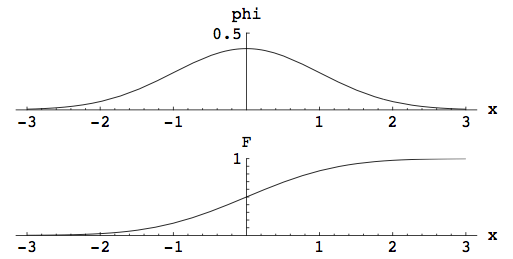
\includegraphics[width=7.5cm]{bilder/normalverteilung.png}
		Dichtefunktion (oben) und Verteilungsfunktion (unten) der Normalverteilung. 
   		\end{minipage} \\ \\
		$ 68\% $ der Werte liegen im Intervall $[ \mu - \sigma, \mu + \sigma]$, 
		$95\% $ in $[ \mu - 2\sigma, \mu + 2\sigma]$, 	
		$99.7\% $ in $[ \mu - 3\sigma, \mu + 3\sigma]$\\\\
		\textbf{ Normalverteilung mit mehreren Unbekannten}\\
		$\varphi_{x,y}(\alpha,\beta)=\frac{1}{2\pi \sigma_x \sigma_y \sqrt{1-\rho_{xy}^2}}
			e^{-\frac{1}{2(1-\rho_{xy})^2} + \frac{(\alpha - m_x)^2}{\sigma_x^2} 
			- 2\rho_{xy}\frac{(\alpha - m_x)\beta - m_y)^2}{\sigma_x \sigma_y} + \frac{(\beta - m_y)^2}{\sigma_y^2}}$\\
			$\varphi_X(\textbf{x})=\frac{1}{(2\pi)^{\frac{n}{2}}|\textbf{C}_x|^{\frac{1}{2}}}\cdot 
			e^{-\frac{1}{2}(\textbf{x} - \textbf{m}_x)^T \textbf{C}_x^{-1} (\textbf{x} - \textbf{m}_x)}$ mit \\
			$\textbf{m}_x=[E(x_1), E(x_2), \ldots, E(x_n)]^T$ und der Kovarianzmatrixe $\textbf{C}_x$; $c_{ij} = E((x_i-E(x_i)(x_j-E(x_j))))$ \\
		\textbf{Rechenregel für die Normalverteilung mit mehreren Unbekannten}
		\begin{itemize}
		  \item wenn $z=a x + b y$ dann ist \\
		  $m_z =  a m_x + b m_y$\\
		  $\sigma_z^2 = a^2\sigma_x^2 + b^2\sigma_y^2+2ab\sigma_x\sigma_y$
		  \item wenn x und y unkorreliert sind, dann ist \\
		  		$f_{x,y}(\alpha, \beta) = \varphi_x(\alpha)\varphi_y(\beta)$ dass heisst x und y sind auch statistisch unabhängig.
		  \item Der optimale nicht lineare Schätzer für die Werte $\mu$ und $\sigma$ ist gleich dem lineare Schätzer.
		\end{itemize}
   		
 
        
        
        
\subsection{Zufallsprozesse}
\begin{minipage}{10.3cm}
	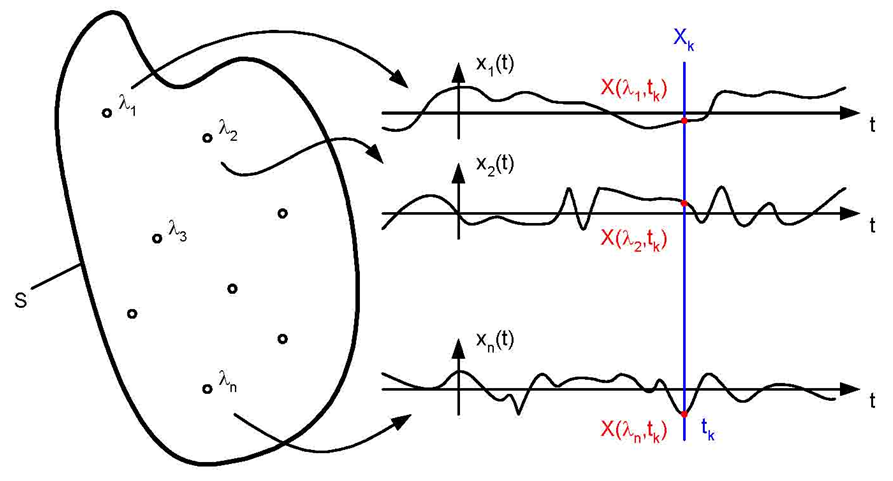
\includegraphics[width=10cm]{bilder/zufallsprozess.png}
\end{minipage}
\begin{minipage}{8.5cm}
	Bei einem \textbf{Zufallsprozess} wird jedem \textbf{Ergebnis} \boldmath$\lambda$ aus 
	dem \textbf{Ergebnisraum} $S$ eine \textbf{deterministische} \textbf{Funktion} $x(\lambda, t)$
	\unboldmath zugewiesen. \\
	Zufallsprozesse beschreiben eine deterministische Zeitfunktion ausgelöst durch ein Ergebnis eines
	Zufallsexperiments. z.B $sin(\omega t + X)$ wobei X eine Zufallsvariable ist, welche zu Beginn aus dem Ereignisraum zugewiesen wird\\
	Zeitlich \textbf{zufällig ablaufende Funktionen} können ebenfalls als \textbf{deterministische} Funktionen 
	\textbf{aufgefasst} werden, bei denen der Beobachter nie weiss, welche Funktion $x_\lambda(t)$ konkret
	vorliegt.	\\ \\
	Zum Vergleich: Bei Zufallsvariablen wird jedem Elementarereignis eine Zahl zugewiesen. 
\end{minipage} 
\vspace{0.5cm} \\

\subsubsection{Statistische Mittelwerte (Scharmittel)}
Die statistischen Mittelwerte sind eine Funktion der Zeit $t$, da es sich um Mittelwerte über das
Ensemble (ganzer Ergebnisraum) handelt. Hierbei werden alle deterministischen Funktionen zu einem
bestimmten Zeitpunkt $t$ gemittelt. 

\renewcommand{\arraystretch}{1.4}
\begin{tabular}[c]{ p{4.5cm}  p{13.5 cm}  }
	\textbf{Erwartungswert}: 	&  $\mu_{x}(t) = E\left[X(t)\right] =
          \int\limits_{-\infty}^{+\infty} x \cdot f_{X}(x;t)\;dx$ bzw $=\frac{1}{N}\sum\limits_{i=1}^{N}x_i(n)$ \\
    \textbf{Erwartungswert eines deterministischen Signals}:& $\mu_f(t) = E(f(t))=f(t)$\\
 	\textbf{Varianz}: &         $\sigma_X^2(t)=E((x(t)-\mu_X(t))^2)=c_X(t_1,t_1)$
    
	 
\end{tabular}
\renewcommand{\arraystretch}{1}


\subsubsection{Stationarität}
Ein stationärer Prozess verändert seine statistischen Eigenschaften über die Zeit nicht. \\

\textbf{Streng Stationär (SSS - Strict Sense Stationary)}\\
% TODO genaue beschreibung streng, schwach stationär
Bei einem streng stationären Prozess bleiben die n-dimensionale WSK-Dichten über die
Zeit konstant. D.h. die \textbf{statistischen Eigenschaften} und somit auch die WSK-Dichten sind zu 
\textbf{allen Zeitpunkten dieselben}.
$$ f_X(x_1, x_2, \ldots, x_n; t_1, t_2, \ldots, t_n) =
		f_X(x_1, x_2, \ldots, x_n; t_1+c, t_2+c, \ldots, t_n+c) \qquad \forall (c,n \in
		\mathbb{R})$$
% Es gelten folgende Beziehungen: \\
% $$E[X(t)] = \mu_{x} \qquad \qquad
% r_{xx}(t_{1},t_{2}) = r_{x}(\tau),\quad \text{ mit } \tau = t_{2} - t_{1} \qquad \qquad
% c_{xx}(t_{1},t_{2}) = r_{x}(\tau) - \mu_{c}^{2}$$ 

\textbf{Schwach Stationär (WSS - Wide Sense Stationary) - Stationarität 2. Ordnung}\\
Bei einem schwach stationären Prozess sind die statistischen Eigenschaften zwar
\textbf{nicht zu jedem Zeitpunkt die selben}, jedoch sind sie \textbf{nicht} von einem \textbf{absoluten} Zeitpunkt, sondern
von der \textbf{Differenz} ($\tau$) \textbf{zweier Zeitpunkte} ($t_1, t_2$) abhängig.  \\ 
$$ f_X(x_1, x_2; t_1, t_2) = f_X(x_1, x_2; t_1+c, t_2+c) \qquad \forall (c \in
		\mathbb{R})$$
%Zudem gilt:\\
\renewcommand{\arraystretch}{1.4}
\begin{tabular}[c]{ p{3.3cm}  p{6.5cm} p{8cm} }
	\textbf{Mittelwert}: 	&  $E[X(t)] = \mu_{x} = \text{const.}$  
							& bleibt über die ganze Zeit konstant\\ 
	\textbf{quad. Mittelwert}: 	&  $E[X^{2}(t)] = r_{x}(0)$  \\ 
	\textbf{Autokorrelation}: 	& 	$r_{xx}(t_{1},t_{2}) = r_{x}(\tau)$
	& \multirow{2}{8cm}{nur \textbf{abhängig} von der \textbf{Zeitdifferenz} $(\tau = t_2 - t_1)$ und \textbf{nicht direkt} von
	 der \textbf{Zeit} $t$} \\
	 \textbf{Autokovarianz}:		& $ c_{xx}(t_{1},t_{2}) = r_{x}(\tau) - \mu_{x}^{2} = c_{xx}(\tau)$ \\
\end{tabular}
\renewcommand{\arraystretch}{1}
 
Bei einem Zufallsprozess handelt es sich immer um ein WSS-Prozess, sobald der Erwartungswert
konstant ist und die Autokorrelationsfunktion nur eine Funktion von $\tau$ ist, d.h. beide 
statistischen Kennwerte bzgl. einer zeitlichen Verschiebung unabhängig sind.    
Jeder streng stationäre Prozess ist auch schwach stationär, aber nicht umgekehrt. 
        
%   \item Zwei Zufallsprozesse heissen Verbund-schwach-station\"ar, wenn jeder Prozess f\"ur sich 
%         schwach-station\"ar ist und zudem gilt:  
%         \begin{itemize}
%           \item[$\circ$] $r_{xy}(t_{1},t+\tau) = E[X(t)Y(t+\tau)] = r_{xy}(\tau)$ 
%         \end{itemize} 
%   \item Dann gilt auch:
%   \begin{itemize}
%      \item[$\circ$] $c_{xy}(\tau) = r_{xy}(\tau) - \mu_{x} \mu_{y}$
%   \end{itemize} 
% \end{itemize} 

%TODO verbund schwach stationär

\subsubsection{Zeitliche Mittelwerte (Zeitmittel)}
Hierbei werden die jeweiligen deterministischen Funktionen (Musterfunktionen) zeitlich gemittelt.
Wird das zeitliche Mittel über den gesamten Zufallsprozess berechnet, so handelt es sich bei den
zeitlichen Mittelwerten um \textbf{Zufallsvariablen}, d.h. die folgenden zwei Ausdrücke sind
abhängig davon (darum Index $_i$), welche Funktion genutzt wird.

%\renewcommand{\arraystretch}{1.4}
\begin{tabular}[c]{ p{4cm}  p{14.5cm}  }
	\textbf{Mittelwert}: 	&  
	$\overline{x_{i}} = \left\langle x_{i}(t) \right\rangle = 
           \lim\limits_{T \rightarrow \infty}
             \frac{1}{T} \int\limits_{-\frac{T}{2}}^{+\frac{T}{2}} x_{i}(t) \; dt$ \\
   	\textbf{Autokorrelation}: 	& 	
   	$\overline{r}_{x_{i}x_{i}}(\tau) = \left\langle x_{i}(t) \cdot x_{i}(t+\tau) \right\rangle = 
           \lim\limits_{T \rightarrow \infty}
             \frac{1}{T} \int\limits_{-\frac{T}{2}}^{+\frac{T}{2}} x_{i}(t) \cdot x_{i}(t + \tau) \; dt$\\
    \multicolumn{2}{l}{Falls der \textbf{Prozess stationär} ist gilt zudem: } \\
	\textbf{Mittelwert}: 	&  
	$E[\overline{x}] = 
           \lim\limits_{T \rightarrow \infty}
             \frac{1}{T} \int\limits_{-\frac{T}{2}}^{+\frac{T}{2}} E[x(t)] \; dt = 
             \frac{1}{T} \int\limits_{-\frac{T}{2}}^{+\frac{T}{2}} \mu_{x} \; dt = \mu_{x}$  \\
   	\textbf{Autokorrelation}: 	& 	
   	$E[\overline{r}_{xx}(\tau)] = 
           \lim\limits_{T \rightarrow \infty}
             \frac{1}{T} \int\limits_{-\frac{T}{2}}^{+\frac{T}{2}} E[x(t)x(t+\tau)] \; dt =
             \frac{1}{T} \int\limits_{-\frac{T}{2}}^{+\frac{T}{2}} r_{xx}(\tau) \; dt = r_{xx}(\tau)$\\
\end{tabular}
\renewcommand{\arraystretch}{1}

\subsubsection{Ergodizität}
Ein stationärer Prozess ist zudem noch ergodisch, wenn die \textbf{zeitlichen Mittelwerten} den
\textbf{statistischen Mittelwerten entsprechen}. %\hspace{2cm} \textbf{Zeitmittel = Scharmittel}\\ 


	\begin{minipage}{5cm}
		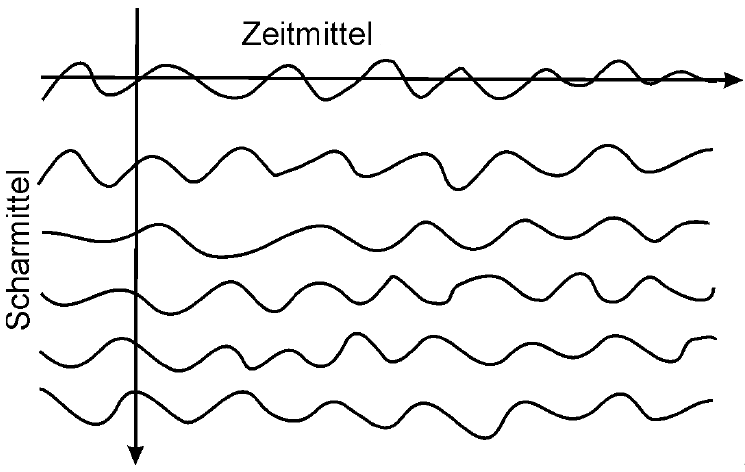
\includegraphics[width=4.5cm]{bilder/zeit-scharmittel.png}
  	\end{minipage}
	\begin{minipage}{13.5cm}

	\begin{tabular}{ll}
  		\multicolumn{2}{l}{Nur bei ergodischen Prozessen gilt zwingend:} \\ \\
      $E[X(t)] = \overline{x} = \left\langle x(t) \right\rangle$ & DC-Level \\
      $E[X(t)]^{2} = (\overline{x})^{2} = \left\langle x(t) \right\rangle^{2}$ & DC-Leistung \\
      $E[X^{2}(t)] = r_{xx}(0) = \overline{x^{2}} = 
                     \left\langle x^{2}(t) \right\rangle $ & Gesamtleistung \\
      $\sigma_{X}^{2}(t) = \left\langle x^{2}(t) \right\rangle 
                           - \left\langle x(t) \right\rangle^{2}$ & AC-Leistung \\
      $\sigma_{X}(t) = \overline{\sigma}_{X}$ & RMS-Level (Effektivwert) des AC-Signals\\
    \end{tabular} \\
  	\end{minipage}


\subsubsection{Vergleich Stationär - Ergodisch}
\textbf{Mückenschwarm:}\\
\textbf{Ergodisch:} Fliegen alle Mücken zusammen in einem Schwarm, so fliegt jede Mücke über die
ganze Zeit gemittelt (Zeitmittel) so schnell wie der ganze Schwarm im Mitel (Scharmittel), ansonsten
würde der Schwarm nicht zusammenhalten können. \\
\textbf{Stationär:} Ist eine Mücke krank und kann mit dem Schwarm nicht mithalten, so fliegt sie
alleine und v.a. langsamer. Somit ist ihre Durchschnittsgeschwindigkeit (Zeitmittel) nicht gleich
derjenigen des Schwarms (Scharmittel), also kommt sie später am Ziel an. \\
\textbf{Weder noch:} Fliegen die Mücken nach dem Start immer langsamer, so ist die
durchschnittliche Geschwindigkeit des Schwarms (Scharmittel) nicht konstant.

\textbf{Schulnoten:}\\
\textbf{Ergodisch:} Alle Schüler müssten dieselbe Zeugnisnote (Zeitmittel) haben und zudem müsste
diese Note jeweils auch dem Klassenschnitt (Scharmittel) der einzelnen Prüfungen entsprechen. \\
\textbf{Stationär:} Der Klassenschnitt (Scharmittel) ist bei jeder Prüfung gleich, jedoch gibt es
unterschiedlich starke Schüler mit unterschiedlichen Zeugnisnoten (Zeitmittel). \\
\textbf{Weder noch:} Der Klassenschnitt (Scharmittel) ist immer unterschiedlich.

\textbf{Thermisches Widerstandsrauschen:} \\
Dies ist bei gleichbleibender Temperatur \textbf{ergodisch}.

\clearpage
\subsubsection{Korrelationen und Leistungsspektren}
Formeln in diesem Abschnitt gelten für \textbf{stationäre} Prozesse. \\

\renewcommand{\arraystretch}{1.6}
\begin{tabular}[c]{ p{3.5cm}  p{6cm} p{7.5cm} }
	\textbf{Autokorrelation}: 	&  
	\multicolumn{2}{l}{$r_x(t_1,t_2)=r_x(t_1-t_2)=r_x(\tau)=r_{xx}(\tau) = E[X(t)X(t+\tau)]$} \\
  	&	$\mid \! r_{xx}(\tau) \! \mid \leq r_{xx}(0) = E[X^{2}(t)]$ 
	& $r_{xx}(-\tau) = r_{xx}(\tau) \quad$ (gerade, Fouriertransformation wird real)\\
  \textbf{Kreuzkorrelation}:& 	
 	$r_{XY}(\tau)=r_{xy}(\tau) = E[X(t)Y(t+\tau)]$  
	& $r_{xy}(-\tau) = r_{yx}(\tau) \quad$ (Reihenfolge Indizes!) \\
    & $|r_{xy}(\tau)| \leq \frac{1}{2} \left[ r_{xx}(0)+r_{yy}(0)\right] $
	& $|r_{xy}(\tau)|  \leq \sqrt{r_{xx}(0)r_{yy}(0)}$ \\
   \textbf{Autokovarianz }: 	&  \multicolumn{2}{l}{$c_{xx}(t_{1},t_{2}) =
          E\left[ \left( X(t_{1})-\mu_{x}(t_{1})\right) \cdot
                  \left( X(t_{2})-\mu_{x}(t_{2})\right) \right] =
          r_{xx}(t_{1},t_{2}) - \mu_{x}(t_{1}) \cdot \mu_{x}(t_{2})=$}\\	
	&\multicolumn{2}{l}{$c_X(\tau)=c_{xx}(\tau) = E\!\left[ \left( X(t)      - E[X(t)]      \right) \cdot
                                  \left( X(t+\tau) - E[X(t+\tau)] \right) \right] =
                        r_{xx}(\tau) - \mu^{2}_{X} $} \\
   	\textbf{Kreuzkovarianz}: 	& \multicolumn{2}{l} {$c_{xy}(t_{1},t_{2}) = 
          E\left[ \left( X(t_{1})-\mu_{x}(t_{1})\right) \cdot
                  \left( Y(t_{2})-\mu_{y}(t_{2})\right)^* \right] =
          r_{xy}(t_{1},t_{2}) - \mu_{x}(t_{1}) \cdot \mu_{y}(t_{2})=$}\\	
   	&\multicolumn{2}{l}{$c_{xy}(\tau) = E\!\left[ \left( X(t)      - E[X(t)]      \right) \cdot
                                  \left( Y(t+\tau) - E[Y(t+\tau)] \right) \right] =
                        r_{xy}(\tau) - \mu_{x}\mu_{y} $}\\
    & \multicolumn{2}{l}{Zufallsprozesse bezeichnet man als zueinander
                        \textbf{unkorreliert}, wenn $c_{xy}(\tau) = 0$}
\end{tabular}
\renewcommand{\arraystretch}{1}

\textbf{Spektrale Leistung}\\
Autokorrelationsfunktion $r_{xx}(\tau)$ und Leistungsspektraldichte $P_{xx}(\omega)$ bilden ein
Fourier-\textbf{Transformationspaar}. \\ Die Leistungsspektraldichte kann als \textbf{mittlere Leistung pro Frequenzband }aufgefasst werden, sie ist
wie folgt definiert:                             
        $$ P_{xx}(\omega) = E\left[ \lim\limits_{T \rightarrow \infty}
                                    \frac{1}{T} \cdot \mid\! X(\omega) \!\mid^{2}\right]                          
                            = \int\limits_{-\infty}^{+\infty} r_{xx}(\tau) \cdot e^{-j\omega\tau} \; d\tau 
                            \qquad \IFT \qquad
        r_{xx}(\tau)   = \frac{1}{2\pi} \int\limits_{-\infty}^{+\infty} 
                             P_{xx}(\omega) \cdot e^{j\omega\tau} \; d\omega$$ bzw:
                             $$P_{xx}(z) = \sum\limits_{k=-\infty}^{\infty} r_{xx}(k)z^{-k}\qquad \IFT \qquad 
                             r_{xx}(k)=\frac 1{2\pi} \int \limits_{-\pi}^{pi} P_{xx}(z)z^k$$
                             
$P_{xx}(\omega)$ ist rein reell, symetriesch $(P_{xx}(z)=P_{xx}^*(\frac{1}{z^*}))$ und $\geq 0$. \\
Kreuzkorrelationen ($r_{yx}(\tau), r_{xy}(\tau)$) und Kreuz-Spektraldichten ($P_{yx}(\tau),
P_{xy}(\tau)$) bilden ein Fourier-Transformationspaar.
\begin{center}
$ r_{yx}(\tau) \FT P_{yx}(\omega) \qquad \qquad r_{xy}(\tau) \FT P_{xy}(\omega)  $
\end{center}
Da die Autokorrelation sicher nicht kausal sind (auch für negative Zeitwerte definiert sind), muss die beidseitige z-Transformation angewendet werden.

Die Eigenwerte der Autokorrelationmatrix haben folgende Begrenzung:\\
$$\min\limits_\omega P_{xx}(z)\leq \lambda_i \leq \max\limits_{\omega}P_{xx}(z)$$

\subsubsection{Beispiele Autokorrelation}
\begin{tabular}{|l|l|l|}
%     \hline
%         \multicolumn{2}{|l|}{\textbf{Beispiele Autokorrelation}} \\
    \hline
        Weisses Rauschen
        & $r_{xx} (n) = \frac {N_0}{2} \delta(n) \FT P_{xx}(z)= \frac {N_0}{2};\hspace{0.25cm}$ & alle z\\
    \hline
        Prozess erster Ordnung
        & $r_{xx} (n) = P_s \cdot a^{|n|} \FT P_{xx} (z) = P_s \cdot \frac {1-a^2}{(1-az^{-1})(1-az)}$ & für $a<|z| < \frac{1}{a}$\\
    \hline
        
        & $r_{xx} (n) = a^n(u(n) - u(n-N)) \FT P_{xx} (z) = \frac{1-a^Nz^{-N}}{1-az^{-1}}$ & für $|z| > 0$\\
    \hline
        
        & $r_{xx} (n) = a^n \cdot u(n) \FT P_{xx} (z) = \frac{1}{1-az^{-1}}$ & für $|z| > a$\\
    \hline
        
        & $r_{xx} (n) = -a^n \cdot u(-n-1) \FT P_{xx} (z) = \frac{1}{1-az^{-1}}$ & für $|z| < a$\\
    \hline
        Binäres Datensignal
        & $r_{xx} (0) = P_s = A_1^2p_1 + A_0^2 p_0 $ &\\
        &$r_{ss} (|n| < T) = $ linearer Übergang von $r_{ss}(0)$ zu $r_{ss} (|n| = T)$ &\\
        & $r_{xx} (|n| \geq T) = P_s = A_1^2p_1^2 + A_0A_1p_0p_1 + A_1A_0p_1p_0 + A_0^2p_0^2$ &  \\
    \hline
        überlagerte Signale
        & $r_{gg\pm}(n) = r_{ss}(n) + r_{sf}(n) + r_{sf}(-n) + r_{ff}(n) $ &\\
        $g_\pm(t) = s(t) \pm f(t)$
        &  $\FT P_{g+}(\omega) = P_{s}(\omega) + P_{f}(\omega) \pm 2 \text{Re} \{P_{sf}(\omega) \}$ &\\ 
    \hline
\end{tabular} 
\vspace{-0.5cm}
\subsubsection{Numerische Berechnung}
\begin{tabular}{|l|l|}
    \hline
		\multicolumn{2}{|l|}{\textbf{Numerische Berechnung}} \\
    \hline
    Autokorrelation
        & $\hat{r}_{xx} (n) = \frac 1 N \sum\limits_{m=0}^{N-1} s(m ) s[(m+n) ] 
                                     = \frac 1 N \sum\limits_{m=0}^{N-1} s[(m-n) ] s(m ) \DFT \hat{P}_{xx}(z)$ \\
    \hline
    Kreuzkorrelation
        & $\hat{r}_{xy} (n ) = \frac 1 N \sum\limits_{m=0}^{N-1} s(m ) f[(m+n) ] 
                                     = \frac 1 N \sum\limits_{m=0}^{N-1} s[(m-n) ] f(m ) \DFT \hat{P}_{xy}(z) $ \\
    \hline
    Leistungsdichtespektrum 
        & $\hat{P}_{xx}(z) = \frac 1N \left|S_T(z)\right|^2 \IDFT \hat{r}_{xx} (n )
            \qquad \text{mit} \quad S_T(z) \IDFT s(n)$\\
    \hline
    Kreuz(leistungsdichte)spektrum 
        & $\hat{P}_{xy}(z) = \frac 1N S_T^*(z) F_T(z) \IDFT \hat{r}_{xy} (n )
        \qquad \text{mit} \quad F_T(z) \IDFT f(n)$\\
				
    \hline
\end{tabular}
\subsubsection{Übertragung von Zufallsprozessen durch LTI-Systeme}
Ein Zufallsprozess wird durch ein LTI-System übertragen. \hspace{2cm} $Y(t) = L[X(t)] \Rightarrow
Y(t) = h(t) \ast X(t)$ \vspace{0.3cm}\\
\renewcommand{\arraystretch}{1.4}
 \begin{tabular}[c]{ p{2cm}  p{8.5cm} p{8cm} }
	& \textbf{Allgemein} & \textbf{WSS-Prozess} \\
	\textbf{Mittelwert}
		& $\mu_{y}(t) = h(t) \ast \mu_{x}(t)$
		& $\mu_{y} = H(0) \mu_{x}$ \\
	\textbf{Auto-korrelation\textcolor{red}{*}}
		& {$r_{yy}(t_{1},t_{2}) = \int\limits_{-\infty}^{+\infty}
		\int\limits_{-\infty}^{+\infty} h(\alpha) h(\beta)
                      r_{xx}(t_{1}-\alpha, t_{2}-\beta) \; d\alpha \; d\beta$}
		& {$r_{yy}(\tau) = \int\limits_{-\infty}^{+\infty}
		\int\limits_{-\infty}^{+\infty} h(\alpha) h(\beta)
                      r_{xx}(\tau+\alpha-\beta) \; d\alpha \; d\beta$} \\
	\textbf{Spektrale Leistung}
		&
		& $P_{yy}(\omega)= H^{\ast}(\omega) H(\omega) P_{xx}(\omega)
			= |H(\omega)|^{2} P_{xx}(\omega)$  \\
\end{tabular}
\renewcommand{\arraystretch}{1} \\
\textcolor{red}{*} = Es ist viel einfacher die Autokorrelation aus der Spektralen Leistung
(Transformationspaar) - anstatt aus diesem höllischen Integral - auszurechnen. \\
Ein WSS-Prozess am Eingang erzeugt auch einen WSS-Prozess am Ausgang.

\subsubsection{Filterung von Zufallsprozessen}
Die Ausgangs Autokorrelation $r_y(k)$ ist\\
 $r_y(k) = r_x(k)\ast h(k) \ast h^*(-k)$ bzw. $\boxed{P_{y}(z) = P_{x}(z)\cdot H(z) \cdot H^*(\frac{1}{z^*}) \quad
  P_{y}(e^{j\omega})=P_x(e^{j\omega})\cdot|H(e^{j\omega})|^2}$

\subsubsection{Weisses Rauschen}
\begin{center}
	\begin{minipage}{8cm}
		$P_{xx}(\omega) = \dfrac{\eta}{2} \qquad r_{xx}(\tau) = \dfrac{\eta}{2} \cdot \delta(\tau)= \sigma_x^2 \cdot \delta(\tau)$ \\ \\
		Beispiel: therm. Rauschen von Widerständen \\
		\textbf{Nimmt} in der Praxis im \textbf{Tera-Hz Bereich ab}!
  	\end{minipage}
	\begin{minipage}{10cm}
		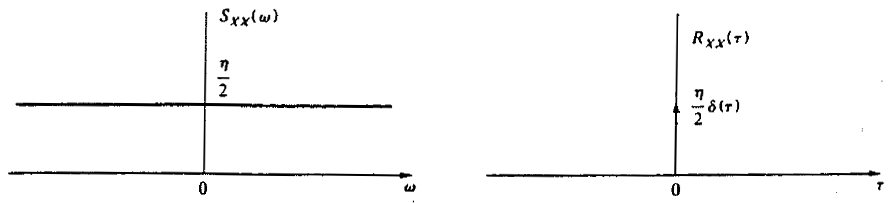
\includegraphics[width=9cm]{bilder/weisses_rauschen.png}
  	\end{minipage}
\end{center}

\subsubsection{Farbige Rauschsignale}
\renewcommand{\arraystretch}{2}
\begin{tabular}[c]{ | p{4cm} | p{3.5cm} | p{3cm} | p{6cm} | }
% 	\hline
% 		Weisses Rauschen
% 		& White Noise
% 		& $P_{xx}(\omega) = \dfrac{\eta}{2}$
% 		& \\
	\hline
		\textbf{Bezeichnung (De)}
		& \textbf{Bezeichnung (En)}
		& \textbf{Leist.-Spektrum}
		& \textbf{Anmerkung} \\
	\hline
		Rosa Rauschen
		& Pink Noise
		& $P_{xx}(\omega) = c \cdot \dfrac{1}{\omega}$
		& Testsignal für Tontechnik, wegen konstanter Leistung pro Oktave \\
	\hline
		Braunes/Rotes Rauschen
		& Brown/Red Noise
		&	$P_{xx}(\omega) = c \cdot \dfrac{1}{\omega^2}$
		& \\
	\hline
		Blaues Rauschen
		& Blue Noise
		&	$P_{xx}(\omega) = c \cdot \omega$
		& \\
	\hline
		Violettes Rauschen
		& Purple/Violet Noise
		&	$P_{xx}(\omega) = c \cdot \omega^2$
		& \\
    \hline
\end{tabular}
\renewcommand{\arraystretch}{1}

\clearpage
\subsection{Estimation \hayes{72}}
  \subsubsection{Bias}
    The bias is the difference between the real value $\Theta$ and the estimate $\hat{\Theta}$: 
    $B = \Theta - E(\hat{\Theta}_N)$. When $B=0$, the estimator is \em unbiased\em. When the estimator
    is biased but the bias goes to zero as the number of observations $N$ goes to infinity, then
    the estimator is \em asymptotically unbiased \em ($\lim_{N \rightarrow \infty} E(\hat{\Theta}_N) = \Theta$). 
    If the bias stays $B \neq 0$, the estimator is \em biased\em.
    
  \subsubsection{Consistency}
    If $\lim_{N \rightarrow \infty} Var(\hat{\Theta}_N) = 0$, the estimator is consistent. 
    $\hat{\Theta}_N$ is said to \em converge to $\Theta$ with probability one\em. 
    Here, a \em consistent \em estimator if it is asymptotically unbiased and has a variance that
    goes to zero as $N$ goes to infinity.
     


\vspace{1em}
\begin{minipage}[t]{10cm}
  \vspace{-2cm}
  \section{Signal Modeling \hayes{129}}
  %\renewcommand{\arraystretch}{1.0}
  \textbf{Ziel: } Die Koeffizienten für ein Filter berechnen, dessen
  Impulsantwort möglichst genau mit einer gegebenen Signal ($x[n]$ - mit
  Länge $n$) übereinstimmt.
      $$ H(z) = \dfrac{B(z)}{A(z)} = \dfrac{b_0 + b_1z^{-1} + b_2 z^{-2} + \dots +
      b_q z^{-q}}{1 + a_1z^{-1} + a_2 z^{-2} + \dots + a_p z^{-p}} $$ 

\end{minipage}
\hspace{0.25cm}
\begin{minipage}{9cm}
	\begin{tabular}{| p{1.4cm} | p{2cm} | p{3.9cm} | }
	    \hline
	    \textbf{Impuls\-antwort}
	    & exakte über\-ein\-stimmung
	    & kleinstes Fehler\-quadrat \\
	    \hline
	    \hline
	    \textbf{LS} 
	    & $[0]$
	    & $[1, n - 1]$\\
	    \hline
	    \textbf{Padé} 
	    & $[0, q + p + 1]$
	    & -\\
	    \hline
	    \textbf{Prony} 
	    & $[0, q]$
	    & $[q + 1, n-1]$ \\
	    \hline
	    \textbf{Shanks} 
	    & $[0]$
	    & $[1, n - 1]$\\
	    &&(zuerst a nach LS dann b. nicht beide zusammen)\\
	    \hline
	\end{tabular}\\
	$q$: Anzahl Nullstellen \hspace{1cm} $p$: Anzahl Polstellen
\end{minipage}

\subsection{Least Square Method \hayes{131}}
Die Koeffizienten \textbf{A und B} werden mit dem kleinsten Fehlerquadrat geschätzt. Da für die Schätzung ein $p+q$ Gleichungssystem aufgelöst 
werden muss, wird dies Methode sehr selten angewendet.\\
\begin{minipage}{8cm}
	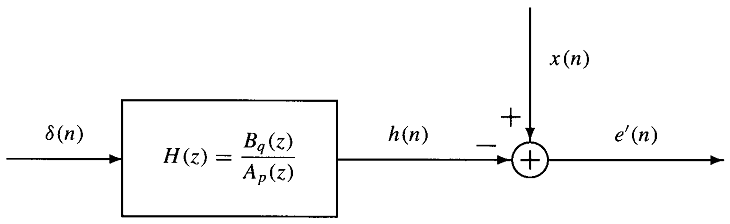
\includegraphics[width=8cm]{../StatDig/bilder/signalModeling.png}
\end{minipage}
\begin{minipage}{10cm}
$\frac{\partial \sum\limits_{n=0}^{\infty}|e'(n)|^2}{\partial a_p^*(k)}=\frac{1}{2\pi} \int\limits_{-\pi}^{\pi}\left[X(e^{j\omega})-
\frac{B_q(e^{j\omega})}{A_p (e^{j\omega})}\right]\frac{B^*_q(e^{j\omega})}{A_p^* (e^{j\omega})^2}e^{j\omega} d\omega=0$\\
$\frac{\partial \sum\limits_{n=0}^{\infty}|e'(n)|^2}{\partial b_q^*(k)}=\frac{1}{2\pi} \int\limits_{-\pi}^{\pi}\left[X(e^{j\omega})-
\frac{B_q(e^{j\omega})}{A_p (e^{j\omega})}\right]\frac{e^{j\omega}}{A_p^* (e^{j\omega})} d\omega=0$\\
\end{minipage} 
\subsubsection{Example FIR Equalizer}
With a FIR first order (2 coefficients) a given sequence (e.g. $[0, 2, 1, 0]$ ) should be filtered so that output is a Dirac $[0, 1 , 0 , 0]$.\\
$\underbrace{\begin{bmatrix}
x[0] 	& 0 	\\
x[1]	& x[0]	\\
0		& x[1]
\end{bmatrix}}_{\bm A}
\cdot \begin{bmatrix}
b_0\\
b_1
\end{bmatrix}=\begin{bmatrix}
1\\
0\\
0
\end{bmatrix}$. To solve the equations the pseudo inverse has to be used: $\bm A^{\dagger} = \left(\bm A^T \cdot \bm A\right)^{-1}\bm A^T 
\Rightarrow \bm  A^\dagger \begin{bmatrix}
1\\
0\\
0
\end{bmatrix}=\begin{bmatrix}
b_0\\
b_1
\end{bmatrix}$

\subsection{Padé Approximation \hayes{133}}
Resultierende Impulsantwort \textbf{stimmt} im Intervall $[0, q + p + 1]$ \textbf{exakt} mit
gegebenem Signal $x[n]$ überein, nachher ist der Filter nicht einmal zwingend stabil.

	%\vspace{-0.5cm}
	\renewcommand{\arraystretch}{1.0}
	\begin{aufzaehlung}
  		\item $a$-Koeffizienten / Pole berechnen: $a_t = - \bm X_t^{-1} \cdot x$ \matlab{$a_t = - X_t \backslash x$} \small $$
	%	\begin{matrix} n=q+1\\ n=q+2\\ \vdots \\ n=q+p \end{matrix}
		\overset{(0 \hdots p)}{\underbrace{\begin{bmatrix}
    		x[q+1] & x[q] & \hdots & x[q+1-p] \\                                   
    		x[q+2] & x[q+1] & \hdots & x[q+2-p] \\
    		\vdots & \vdots & \ddots & \vdots \\                             
    		x[q+p] & x[q+p-1] & \hdots & x[q] \\
		\end{bmatrix}  }_{\bm X}} \cdot \underbrace{\begin{bmatrix}
    		1 \\
    		a_1 \\
    		\vdots \\
    		a_p
		\end{bmatrix}  }_{a} = \begin{bmatrix}
    		0 \\
    		0 \\
    		\vdots \\
    		0
		\end{bmatrix} \Longleftrightarrow 
		\underbrace{ \begin{bmatrix}
    		x[q]     & x[q-1]   & \hdots & x[q-p+1] \\                                   
    		x[q+1]   & x[q]     & \hdots & x[q-p+2] \\
    		\vdots   & \vdots   & \ddots & \vdots \\                             
    		x[q+p-1] & x[q+p-2] & \hdots & x[q] \\
		\end{bmatrix}  
		}_{\bm  X_t} \cdot 
		\underbrace{\begin{bmatrix}
    		a_1 \\
    		a_2 \\
    		\vdots \\
    		a_p
		\end{bmatrix}  }_{a_t} = \underbrace{\begin{bmatrix}
    		-x [q+1]\\            
    		-x [q+2]\\
    		\vdots \\
    		-x [q+p]\\
		\end{bmatrix}}_{x} $$  \normalsize
		
		\vspace{-0.5cm}
		Falls A singulär ist, war die Annahme, dass $a_0 = 1$ falsch. $\Longrightarrow$ $a_0=0$ setzen. 
		$ \Longrightarrow \bm X_t \cdot \bm a_t = \bm 0$
		
  		\item $b$-Koeffizienten / Nullstellen berechnen: $b = \bm X_0 \cdot a$ \small \hspace{0.5cm}
		$ \begin{matrix} n=0\\ n=1\\ \vdots\\ n=q \end{matrix} \overset{(0 \hdots p)}{\underbrace{\begin{bmatrix}
    		x[0] & 0 & \hdots & 0 \\
    		x[1] & x[0] & \hdots & 0 \\
    		\vdots & \vdots & \ddots & \vdots \\
    		x[q] & x[q-1] & \hdots & x[q-p]
		\end{bmatrix}  }_{\bm X_0}}\cdot \underbrace{\begin{bmatrix}
    		1 \\
    		a_1 \\
    		\vdots \\
    		a_p
		\end{bmatrix}  }_{a}= 	\underbrace{\begin{bmatrix}
	    		b_0 \\
	    		b_1 \\
	    		\vdots \\
	    		b_q
			\end{bmatrix}}_{b}$ \normalsize
			
	\end{aufzaehlung}
	
\vspace{-1.0cm}


\subsection{Prony's Method \hayes{144}}
Resultierende Impulsantwort \textbf{stimmt} im Intervall $[0, q]$ \textbf{exakt} mit
gegebenem Signal $x[n]$ überein. Im Intervall $[q + 1, n-1]$ sind die
Werte mit dem \textbf{kleinsten Fehlerquadrat} (überbestimmtes GL-System)
angenähert. 

\renewcommand{\arraystretch}{1.0}

\begin{aufzaehlung}
	\item Autokorrelation berechnen: $ r_x(k,l) = \sum\limits_{n=q+1}^\infty x(n-l)x^*(n-k)$;\qquad $k,l\geq l$
	\item $a$-Koeffizienten berechnen : $a_t = - \bm R_t^{-1} \cdot x$ 
  		\matlab{$a_t = A_t \backslash x$} \small\\
		Der minimale Fehler ist: $\epsilon_{p,q} = r_x(0,0) + \sum\limits_{k=1}^p a_k r_x(0,k)$
			$$
		{\underbrace{\begin{bmatrix}
    		r_x[0,0] & r_x[0,1] & \hdots & r_x[0,p] \\ 
    		----&----&----&----\\
    		r_x[1,0] & r_x[1,1] & \hdots & r_x[1,p] \\                                   
    		r_x[2,0] & r_x[2,1] & \hdots & r_x[2,p] \\
    		\vdots & \vdots & \ddots & \vdots \\                             
    		r_x[p,0] & r_x[p,1] & \hdots & r_x[p,p] \\                        
		\end{bmatrix}  }_{\bm R_t}} \cdot \underbrace{\begin{bmatrix}
    		1 \\
    		a_1 \\
    		\vdots \\
    		a_p
		\end{bmatrix}  }_{a_t}= \begin{bmatrix}
    		\epsilon_{p,q} \\
    		---\\
    		0 \\
    		\vdots \\
    		0
		\end{bmatrix} $$ 
		Für All-Pole Modelle können die a-Koeffizienten direkt aus dem b Gleichungsystem berechnet werden. 
		Dafür müssen alle $b$-Koeffizienten bis auf $b_0$ auf 0 gesetzt werden.
	\item $b$-Koeffizienten berechnen wie bei \textbf{Padé}: $b = \bm X_0 \cdot a$ 
		\normalsize
\end{aufzaehlung}
	
\subsection{Shanks' Method \hayes{154}}

Die B Koeffizient werden bei gegebenen A's so geschätzt, dass die resultierende Impulsantwort ist im Intervall $[0, n - 1]$ mit dem
\textbf{kleinsten Fehlerquadrat} (überbestimmtes GL-System) dem gegebenen
Signal $x[n]$ angenähert wird. Die einzige Verbesserung wäre noch wenn die A- Koeffizenten auch noch alle Signalwerte einbeziehen würden (Least-square).

\begin{aufzaehlung}
  		\item $a$-Koeffizienten berechnen wie bei \textbf{Prony}: $a_t = \bm X_t^{-1} \cdot x$ \matlab{$a_t = X_t \backslash x$}  
  		\item Impulsantwort $g[n]$ des rein rekursiven Filters ($g[n] = \delta(n)- \sum\limits_{k=1}^p a_p(k)g(n-k)$) berechnen, 
  		oder mittels inversen z-Transformation von $H(z)$.
  		\item Autokorrelation berechenen:  $r_g(k-l)=\sum\limits_{n=0}^\infty g(n-l)g^*(n-k)$; oder inverse z-Transformation von $|H(z)|^2$
  		\item Kreuzkorrelation berechnen: $r_{xg}(k-l)=\sum\limits_{n=0}^\infty x(n-l)g^*(n-k)$
  		\item $b$-Koeffizienten berechnen (für stationäre Prozesse): $b = R^{-1} \cdot r_{xg}$ \matlab{$b = C \backslash x$}\\
  		für\\
  		
			
		 $$\begin{matrix}n=0\\ n=1\\ \vdots\\ n=N_{ha}+q\\ \end{matrix}
		\overset{(0 \hdots q)}{\underbrace{\begin{bmatrix}
    		r_g(0) & r_g(1) & \hdots & r_g(q) \\                                            
    		r_g(1) & r_g(0) & \hdots & r_g(q-1) \\         
    		\vdots & \vdots & \ddots & \vdots \\                                      
    		r_g(q) &r_g(q-1) & \hdots & r_g(0) \\    
		\end{bmatrix}  }_{R}} \cdot \underbrace{\begin{bmatrix}
    		b_0 \\
    		b_1 \\
    		\vdots \\
    		b_q
		\end{bmatrix}  }_{b}= \underbrace{\begin{bmatrix}
    		r_{xg}(0) \\
    		r_{xg}(1) \\
    		\vdots \\
    		r_{xg}(q) \\
		\end{bmatrix}  }_{x} $$   \normalsize
\end{aufzaehlung}

\clearpage
\subsection{Approximation mit begrenzten  Daten mit All-Pole Filter}
\subsubsection{Autocorrelation Method \hayes{178}}
Sind die die Autokorrellationen gegeben, siehe Kapitel \ref{sec:autoregressive_model_method}.\\
Annahme: Die Daten $x[n]$ sind ausserhalb des Definitionsbereichs ($n=[0..N]$) Null: $x[n]=0$. So wird der Filter in einen stabilen Zustand gezwungen.
\renewcommand{\arraystretch}{1.0}

\begin{aufzaehlung}
	\item $a$-Koeffizienten berechnen (mittels Pseudoinverse / generalisierte Inverse): $a_t = \left(\bm X_t^T \cdot \bm  X_t\right)^{-1} \cdot \bm X_t^T \cdot x$
  		\matlab{$a_t = X_t \backslash x$} \small
			$$
		\begin{matrix} n=q+1\\ n=q+2\\ \vdots \\ n=N\\ n=N+1\\ \vdots \\ N+p
		\end{matrix}
		\underbrace{\begin{bmatrix}
    		x[0] & 0 & \hdots & 0 \\ 
    		x[1] & x[0] & \hdots & 0 \\ 
    		x[2] & x[1] & \hdots & 0 \\        
    		\vdots & \vdots & \ddots & \vdots \\
    		----&----&----&----\\                
    		x[p-1] & x[p-2] & \hdots & x[0] \\                                   
    		x[p] & x[p-1] & \hdots & x[1] \\      
    		\vdots & \vdots & \ddots & \vdots \\                        
    		x[N-1] & x[N-2] & \hdots & x[N-p] \\ 
    		----&----&----&----\\                            
    		x[N] & x[N-1] & \hdots & x[N-p+1] \\ 
    		0 & x[N] & \hdots & x[N+2-p] \\
    		\vdots & \vdots & \ddots & \vdots \\                     
    		0 & 0 & \hdots & x[N] \\
		\end{bmatrix}  }_{\bm X_t=(N+p \; \times \; p) Matrixe} \cdot \underbrace{\begin{bmatrix}
    		1 \\
    		a_1 \\
    		\vdots \\
    		a_p
		\end{bmatrix}  }_{a_t}= \underbrace{\begin{bmatrix}
    		 -x [1]\\            
    		 -x [2]\\
    		\vdots \\
    		 -x [N]\\
    		0 \\
    		\vdots \\
    		0
		\end{bmatrix}}_{x} 
		 $$ \normalsize
	\end{aufzaehlung}
	
\subsubsection{Covariance Method  \hayes{183}}
Es werden keine Annahmen getroffen, nur die vorhanden Daten werden verwendet. Der Nachteil ist, dass das Filter instabil werden kann. 
Ein weiterer Nachteil ist, dass A keine Toeplitz Matrixe ist, so dass das Auflösen nicht so einfach ist wie bei der Autokorrelation Methode. 
Das Signal wird jedoch genauer rekonstruiert. Bei einer Datenreihe, welche einer Impulsantwort entspricht, wird der Filter perfekt rekonstruiert. 
Mit dem Nachteil, dass auch die instabilen Pole implementiert werden. $ a_t= \bm X_t^{-1}\cdot x$ \matlab{$a_t = A_t \backslash x$} \small
		$$
		\underbrace{\begin{bmatrix}               
    		x[p-1] & x[p-2] & \hdots & x[0] \\                                   
    		x[p] & x[p-1] & \hdots & x[1] \\      
    		\vdots & \vdots & \ddots & \vdots \\                        
    		x[N-1] & x[N-2] & \hdots & x[N-p] \\ 
		\end{bmatrix}  }_{\bm X_t} \cdot \underbrace{\begin{bmatrix}
    		1 \\
    		a_1 \\
    		\vdots \\
    		a_p
		\end{bmatrix}  }_{a}= \underbrace{\begin{bmatrix}
    		 -x[p+1]\\            
    		 -x[p+2]\\
    		\vdots \\
    		 -x[N]\\
		\end{bmatrix}}_{x} 
		 $$ \normalsize
\vspace{-0.5cm}

\subsection{Stochastische Modelle}
Bei stochastischen Modellen werden generell die gleichen Modelle verwendet, wie in der deterministischen Welt. 
Anstatt des Dirac-Impulses wird weisses Rauschen am Eingang des Filters verwendet und die Autokorrelation wird mit Hilfe des Erwartungswertes gebildet. 
$r(k)=E\{x(n) \cdot x^*(n-k)\}$\\
Anstatt der Kreuzkorellation $r_{gx}$ wird die Faltung von $b_q(k)$ und $h^*(-k)$ verwendet. $c_q(k) = b_q(k) \ast h^*(-k)$

\subsubsection{Autoregressive Moving Average Models, ARMA \hayes{189}}
Ein ARMA Pozess ist weisses Rauschen welches durch ein LTI- System $H(z)$ gefiltert wird.\\
Um die Koeffizienten von $H(z)=\frac{B_q(z)}{A_p(z)}=\frac{\sum\limits_{k=0}^q b_q(k)z^{-k}}{1+\sum\limits_{k=1}^p a_p(k)z^{-k}}$ werden 
die \textbf{erweiterten Yule-Walker Gleichungen} gelöst:
\small$$
\underbrace{\begin{bmatrix}               
    		r_x[0] & r_x^*[1] & \hdots & r_x^*[p] \\   
    		r_x[1] & r_x^*[2] & \hdots & r_x^*[p-1] \\   
    		\vdots & \vdots & \ddots & \vdots \\     
    		r_x[q] & r_x[q-1] & \hdots & r_x[q-p] \\   
    		r_x[q+1] & r_x[q] & \hdots & r_x[q-p+1] \\    
    		\vdots & \vdots & \ddots & \vdots \\     
    		r_x[L] & r_x[L-1] & \hdots & r_x[L-p] \\ 
		\end{bmatrix}  }_{R} \cdot \underbrace{\begin{bmatrix}
    		1\\
    		a_p(1) \\
    		a_p(2) \\
    		\vdots \\
    		a_p(p)
		\end{bmatrix}  }_{a_p}= \begin{bmatrix}
    		 c_q[0]\\            
    		 c_q[1]\\
    		\vdots \\
    		 c_q[q]\\
    		 0\\
    		\vdots \\
    		 0\\
		\end{bmatrix} 
		 $$ \normalsize

\begin{aufzaehlung}
  		\item Berechnen der A- Koeffizienten: $R_q \cdot a_p = - r_{q+1}$
  		\small$$
\underbrace{\begin{bmatrix}                   
    		r_x[q] & r_x[q-1] & \hdots & r_x[q-p+1] \\   
    		r_x[q+1] & r_x[q] & \hdots & r_x[q-p+2] \\    
    		\vdots & \vdots & \ddots & \vdots \\     
    		r_x[q+p-1] & r_x[q+p-2] & \hdots & r_x[q] \\ 
		\end{bmatrix}  }_{R_q} \cdot \underbrace{\begin{bmatrix}
    		a_p(1) \\
    		a_p(2) \\
    		\vdots \\
    		a_p(p)
		\end{bmatrix}  }_{a_p}= \underbrace{\begin{bmatrix}
    		 -r_x[q+1]\\            
    		 -r_x[q+2]\\
    		\vdots \\
    		 -r_x[q+p]\\
		\end{bmatrix}}_{r_{q+1}} 
		 $$ \normalsize
		 \item Zur Berechnung der B- Koeffizienten muss der Umweg über die C- Koeffizienten genommen werden: $R_x \cdot a_p = c_q$
	
  		\small$$
\underbrace{\begin{bmatrix}                   
    		r_x[0] & r_x^*[1] & \hdots & r_x^*[p] \\   
    		r_x[1] & r_x[0] & \hdots & r_x^*[p-1] \\    
    		\vdots & \vdots & \ddots & \vdots \\     
    		r_x[q] & r_x[q+1] & \hdots & r_x[0] \\ 
		\end{bmatrix}  }_{R_x} \cdot \underbrace{\begin{bmatrix}
    		a_p(1) \\
    		a_p(2) \\
    		\vdots \\
    		a_p(p)
		\end{bmatrix}  }_{a_p}= - \underbrace{\begin{bmatrix}
    		 c_q[0]\\            
    		 c_q[1]]\\
    		\vdots \\
    		 c_q[q]\\
		\end{bmatrix}}_{c_{q}} 
		 $$ \normalsize	 
		 \item $[C_q(z)]_+$ aufschreiben: $[C_q(z)]_+ = \sum\limits_{k=0}^q c_q(k)z^{-k}$
		 \item $[P_y(z)]_+=\left[[C_q(z)]_+ \cdot A^*_p(1/z^*)\right]_+$ berechnen. \\
		 z.B $[C_1(z)]_+=\frac{45}{2}-6z^{-1}$, $A^*_p(1/z^*)=1-0.5z$; $[C_1(z)]_+ \cdot A^*_p(1/z^*)= -\frac{45}{4}z +\frac{51}{2}-6z^{-1}$ $\Rightarrow$  $[P_y(z)]_+= \frac{51}{2}-6z^{-1}$
		 \item $[P_y(z)]_+$ symterisch machen. z.B: $P_y(z) =  -6 z +\frac{51}{2}-6z^{-1}$
		 \item Faktorisieren von $P_y(z)=B_q(z)B_q^*(1/z^*)$ damit $B_p(z)$ verwendet werden kann: \\
		 z.B. $B_1(z)\cdot B_1^*(1/z^*)= \underbrace{2\sqrt{6}(1-\frac{1}{4}z^{-1})}_{B_q(z)}\cdot \underbrace{2\sqrt{6}(1-\frac{1}{4}z^{1})}_{B_q^*(1/z^*)}$
		 \item $H(z)=\frac{B_q(z)}{A_p(z)}$ z.B: $H(z)=\frac{2 \sqrt{6}(1-\frac 1 4 z^{-1})}{A_p(z)}$
\end{aufzaehlung}
		 
\subsubsection{Autoregressive Models - AR \hayes{194}}
\label{sec:autoregressive_model_method}
Bei der AR wird die ARMA Methode verwendet, jedoch nur mit Polen. $H(z)=\frac{b(0)}{1+\sum\limits_{k=1}^{p} a_p(k)z^{-k}}$.\\
 $$\begin{bmatrix} 
	 	r_x(0)  & r_x^*(1) & r_x^*(2) & \cdots & r_x^*(p-1)\\
	 	r_x(1)  & r_x(0) & r_x^*(1) & \cdots & r_x^*(p-2)\\
	 	r_x(2)  & r_x(1) & r_x(0) & \cdots & r_x^*(p-3)\\
	 	\vdots  & \vdots  & \vdots  & \vdots & \vdots\\
	 	r_x(p-1)& r_x(p-2)& r_x(p-3)& \cdots &  r_x(0)\\
   \end{bmatrix}=
   \begin{bmatrix}
    	a_p(1)\\
    	a_p(2)\\
    	a_p(3)\\
    	\vdots\\
    	a_p(p)\\
   \end{bmatrix}=
   \begin{bmatrix}
       	-r_x(1)\\
       	-r_x(2)\\
       	-r_x(3)\\
       	\vdots\\
        -r_x(p)\\
   \end{bmatrix}
 $$
 Mit $|b(0)|^2=r_x(0) + \sum\limits_{k=1}^{p} a_p(k)r_x(k)$
 

 
 \subsubsection{Moving Average Models - MA \hayes{195}}
Ein MA Prozess ist eine Spezialform von einem ARMA Prozess, welcher nur Nullstellen besitzt.\\
$P_x(z)=\sum\limits_{k=-q}^{q}r_x(k)z^{-k}=B_q(z)B_q^*(1/z^*)$
\begin{aufzaehlung}
	\item $P_x(z)$ spektral faktorisieren in: $P_x(z)=\sigma^2_0 \cdot Q(z)\cdot Q^*(1/z^*)=\underbrace{\sigma^2_0}_{|b_q(0)|^2} \underbrace{\prod\limits_{k=1}^q (1-\beta_k z^{-1})}_{B_q(z)} \cdot \underbrace{\prod\limits_{k=1}^q (1-\beta_k^* z)}_{B^*_q(1/z^*)}$
	\item $B_q(z)$ ausmultiplizieren $\Rightarrow$ minimum phase filter (alle Nullstellen sind innerhalb des Einheitskreis)
	\item bzw. $B_q^*(1/z^*)$ ausmultiplizieren ergibt ein maximum phase filter (alle Nullstellen sind ausserhalb des Einheitskreis)
\end{aufzaehlung}


\section{Optimum Filters}
A optimum filter minimize the mean-square error $\xi = E\left(|e(n)|^2\right) \quad x(n)=d(n)+v(n) \quad e(n) = d(n) - \tilde{d}(n)$\\
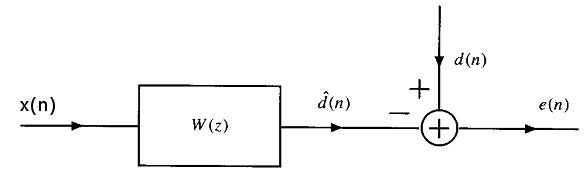
\includegraphics[width=9cm]{../StatDig/bilder/optimumFilter.jpg}\\
The minimal error is \textbf{always orthogonal} to the data: $E(e(n)x^*(n-k))=0$ $\forall$ $k\epsilon[0,p-1]$

\subsection{Wiener FIR Filter \hayes{337}}
\begin{minipage}{10cm}
\begin{tabbing}

Wiener-Hopf equations: \= $\sum \limits_{l=0}^{p-1} w(l)r_x(k-l)=r_{dx}(k)$; $\forall$ $k\epsilon[0,p-1]$ \\
Correlations:  \>
						$r_x(k)=E \{ x(n)x^{*}(n-k) \}$ \\
\>						$r_{dx}(k)=E\{d(n)x^{*}(n-k)\}$ \\
Minimum Error: \>		$\xi_{min}=r_d(0)-\sum \limits_{l=0}^l w(l)r_{dx}^{*}(l)$
\end{tabbing}
\end{minipage}
\begin{minipage}{10cm}
$\small
\underbrace{\begin{bmatrix}                   
    		r_x[0] & r_x^*[1] & \hdots & r_x^*[p-1] \\   
    		r_x[1] & r_x[0] & \hdots & r_x^*[p-2] \\    
    		\vdots & \vdots & \ddots & \vdots \\     
    		r_x[p-1] & r_x[p-2] & \hdots & r_x[0] \\ 
		\end{bmatrix}  }_{R_x} \cdot \underbrace{\begin{bmatrix}
    		w(0) \\
    		w(1) \\
    		\vdots \\
    		w(p-1)
		\end{bmatrix}  }_{w}= \underbrace{\begin{bmatrix}
    		 r_{dx}[0]\\            
    		 r_{dx}[1]\\
    		\vdots \\
    		 r_{dx}[p-1]\\
		\end{bmatrix}}_{r_{dx}} 
		 $$ \normalsize	 $\\
$$R_x \cdot w =r_{dx}$$
\end{minipage}
\begin{minipage}{7.5cm}
\subsubsection{Filtering \hayes{339}}
The input signal is $x(n)=d(n)+v(n)$. Because the noise and the data signal is uncorrollated and the noise has zero mean, the Wiener-Hopf equation simplify follow:\\
$r_x(k)=r_d(k)+r_v(k)$\\
$r_{dx}(k)=r_d(k) \hspace{1.5cm} \rightarrow [R_d + R_v]\cdot w = r_d$\\
 with $R_v=\small \begin{bmatrix}                   
    		\sigma_v^2 & \hdots & 0\\   
    		\vdots & \ddots & \vdots \\     
    		0&  \hdots &\sigma_v^2 \\ 
		\end{bmatrix} $
\end{minipage}
\hspace{5mm}
\begin{minipage}{10cm}
\subsubsection{Linear Prediction FIR \hayes{342}}
$\hat{x}(n+\alpha)=\sum \limits_{k=0}^{p-1} w(k)[x(n-k)+v(n-k)]$

$ 	\hookrightarrow  	\small \begin{bmatrix}                   
    		r_y[0] & r_y^*[1] & \hdots & r_y^*[p-1] \\   
    		r_y[1] & r_y[0] & \hdots & r_y^*[p-2] \\    
    		\vdots & \vdots & \ddots & \vdots \\     
    		r_y[p-1] & r_y[p-2] & \hdots & r_y[0] \\  
		\end{bmatrix}   \cdot \begin{bmatrix}
    		w(0) \\
    		w(1) \\
    		\vdots \\
    		w(p)
		\end{bmatrix} = \begin{bmatrix}
    		 r_{x}[\alpha]\\            
    		 r_{x}[\alpha+1]\\
    		\vdots \\
    		 r_{x}[\alpha+q]\\
		\end{bmatrix}
$$ \normalsize	 $\\
$\alpha$ are the steps to predict. Noise: $r_y(k) = r_x(k) + r_v(k)$\\
\end{minipage}\\
\begin{minipage}{11.5cm}
\subsubsection{Linear Phase Filter \hayes{17}, exercise 9.16} 
All frequency are delayed same. \\
For \textbf{FIR}: the coefficients are symmetric $(z^1+2z^0+z^{-1})$ or with a causal filter: $z^0 + 2z^{-1} + z^{-2}$\\
$\small \begin{bmatrix}
2 r_x[0] + 2 r_x[2]		&	2 r_x[1] \\
2 r_x[1]				& 	r_x[0]
\end{bmatrix} \cdot \begin{bmatrix}
w_n(1)\\
w_n(0)
\end{bmatrix}= \underbrace{ \begin{bmatrix}
r_x[\alpha] + r_x[\alpha+2]\\
r_x[\alpha+1]
\end{bmatrix}}_{\text{for linear prediction} } 
= \underbrace{ \begin{bmatrix} = 
r_{dx}[0] + r_{dx}[2]\\
r_{dx}[1]
\end{bmatrix}    }_{\text{for optimal filter} }  $

\end{minipage}
\hspace{3mm}
\begin{minipage}{7cm}
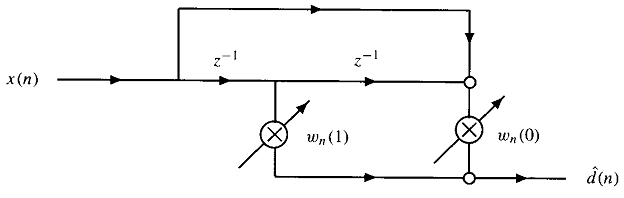
\includegraphics[width=7cm]{../StatDig/bilder/linear_phase_fir.png}
How a linear phase FIR filter 2 order is implemented in hardware.
\end{minipage}
\subsection{Wiener IIR Filter}
\begin{minipage}{8cm}
\subsubsection{Noncausal \hayes{353}}
\begin{tabbing}
Wiener-Hopf equations: \=
$H(e^{jw})=\frac{P_{dx}(e^{jw})}{P_{x}(e^{jw})}  \Rightarrow
\frac{P_{d}(e^{jw})}{P_{d}(e^{jw}) + P_{v}(e^{jw})}= \frac{SNR(e^{j\omega})}{SNR(e^{j\omega}) + 1}$ (often called \textbf{the} Wiener Filter) \\

Correlations: \>
	$r_x(k) =E \{ x(n)x^{*}(n-k) \} $\\ 
	\>$r_{dx}(k) =E\{d(n)x^{*}(n-k)\}$\\


Minimum Error:\>
	$\xi_{min} =r_d(0)-\sum \limits_{l=-\infty}^\infty h(l)r_{dx}^{*}(l)
	=\frac{1}{2\pi}\int \limits_{-\pi}^\pi[P_d(e^{jw})-H(e^{jw})P_{dx}^{*}(e^{jw})]dw$\\
	\>$=r_d(0)-\frac{1}{2\pi}\int \limits_{-\pi}^\pi[H(e^{jw})P_{dx}^{*}(e^{jw})]dw$
\end{tabbing}

\end{minipage}

\subsubsection{Causal \hayes{358}}
\begin{tabbing}
Spectral Factorization: \=
$ P_x(z) = \sigma_0^2 Q(z) Q^*(z^{-1}) $\\

System function:\hspace{1.2cm}\>
	$H(z)=\frac{1}{\sigma_0^2 Q(z) } [\frac{P_{dx}(z)}{Q^*(z^{-1})} ]_+ $ \\
	
Minimum Error:\>$\xi_{min} =r_d(0)-\sum \limits_{l=0}^\infty h(l)r_{dx}^{*}(l)
	=\frac{1}{2\pi}\int \limits_{-\pi}^\pi[P_d(e^{jw})-H(e^{jw})P_{dx}^{*}(e^{jw})]dw$\\
	
\end{tabbing}
Example \hayes{362}

\subsubsection{Linear Prediction IIR \hayes{365}}
\begin{tabbing}
System function:\hspace{0.2cm}\=
	$ r_{dx}(k)=r_x(k+\alpha)  \qquad \alpha \text{ = steps to predict.} $\\
\>	$ H(z)= \frac{1}{Q(z)}[z^\alpha Q(z)]_+ $ \hspace{6.8cm} \=$\rightarrow \text{monic, one step } H(z) = z [1- \frac{1}{Q(z)}] $\\
Minimum Error:\>
	$\xi_{min} =r_d(0)-\sum \limits_{l=0}^\infty h(l)r_{dx}^{*}(l)
		=\frac{1}{2\pi}\int \limits_{-\pi}^\pi[P_d(e^{jw})-H(e^{jw})P_{dx}^{*}(e^{jw})]dw $\>$ \rightarrow \text{monic, one step } \xi_{min} = \sigma^2_0$\\
\end{tabbing}


\subsubsection{Wiener Deconvolution \hayes{369}}
Deconvolutate a signal $x(n)=d(n)\ast g(n) + w(n)$ (not $x(n)=d(n) + g(n)$) it's not easy. At the best, the signal could be reconstruct as:
$\hat{D}(e^{\omega})=D(e^{j\omega}) + \frac{W(e^{j\omega})}{G(e^{j\omega})}=D(e^{j\omega})+V(e^{j\omega})$ \quad $V(e^{j\omega})$ isn't anymore white noise. 
Espacialy if $G(e^{j\omega})$ becomes small the noise will be amplified.\\
System function:\hspace{1.2cm}
	$ H(z)= \frac{1}{G(z)}\left[\frac{P_d(z)}{P_d(z)+P_w(z)/|G(z)|^2}\right]$\\

\subsection{Discrete Kalman Filter \hayes{371}}
The Kalman Filter is a Best Linear Unbiased Estimator (BLUE).

\textbf{Grundgedanke} Beim Kalman Filter wird der Kalman Gain nach dem
kleinsten Fehlerquadrat geschätzt. Speziell am Kalman ist, dass Messgrössen
mithilfe der Zustandsgrössen und einem Rauschsignal definiert ist. \\
\subsubsection{Voraussetzung}
\begin{aufzaehlung}
   	\item Physikalisches Modell/Systementwicklung (für normales sogar ein
   	lineares Modell)
   	\item Messwerte, auch eine Sensorfusion möglich (mehrere Messwerte für ein
   	Systemzustand)
   	\item für normales Kalman: linearer Zusammenhang zwischen Messwerten und
   	Zustandsgrössen
\end{aufzaehlung}
\begin{minipage}{8cm}
	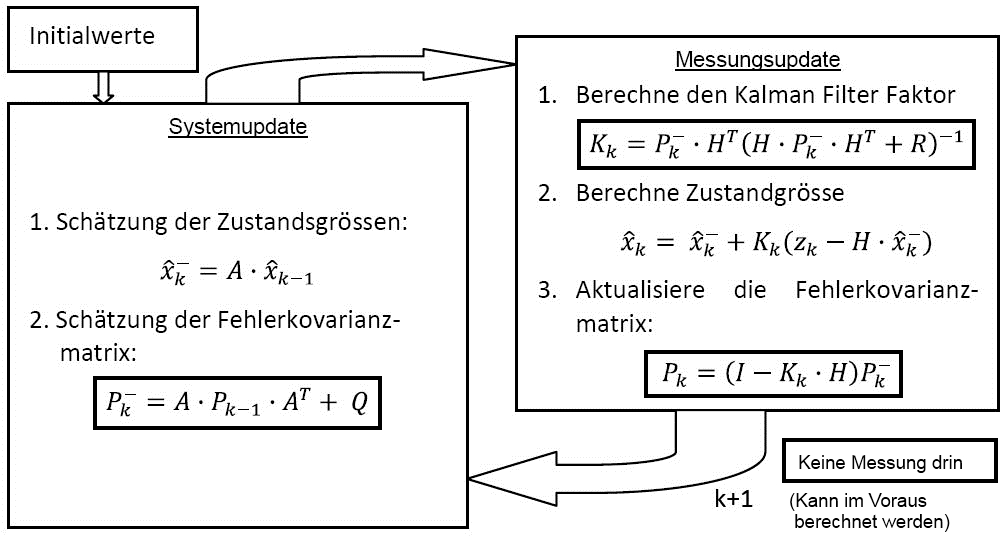
\includegraphics[width=8cm]{Content/AdaptSigVer/KalmanFilter.jpg}
	
	\begin{itemize}
		\item $\hat{x}_{k-1}$ und $P_{k-1}$ benötigen Initialisierungswerte
		\item $P_K$ und $K_K$ können offline vorausberechnet werden, wenn das System nicht ändert
	\end{itemize}
	
\end{minipage}
\begin{minipage}{11cm}
	\small
	\subsubsection{Funktion}
		\begin{liste}
	    	\item A Systementwicklungsmatrize: Physikalische Modell
	    	\item K Kalman Gain: Gewichtet interne Schätzung und die Messungen der
	    	einzelnen Sensoren (0=Nur interne Schätzung;1=nur Messung)
	    	\item H Messmatrize: Zusammenhang zwischen Mess- und Zustandsgrössen
	    	\item P (Fehlerkovarianzma.) Schätzgrösse für den Fehler. Je grösser desto
	    	mehr wird aktuelle Messung berücksichtigt. Beim normalen Kalman Filter
	    	konvergiert dieser mit der Zeit.
	    	\item z: Messwerte (auch von mehreren gleichartigen Sensoren möglich)
	    	\item x: Zustandsgrössen
	    	\item Initialwert: Systemwerte beliebig; Fehlerkovarianzmatrize sehr
	    	gross wählen, so dass zuerst nur die Messung berücksichtigt wird
	    	\item Q Standartabweichung System (Systemrauschen)
	    	\item R Standartabweichung der Sensoren (Messrauschen)
				\item Das Verhältniss von Q zu R ist für die Filtereinstellung verantwortlich.\newline
				$\frac QR$ gross $\rightarrow$ vertraut mehr den Messdaten\newline \hspace{4cm} $\frac QR$ klein $\rightarrow$ vertraut mehr den Systemeigenschaften
	    \end{liste}
	\normalsize
\end{minipage}\\
\clearpage

\subsubsection{Kalman Algorithm}
Idea: Best estimation when process and observer equation as well as some initial conditions are given.
$\mathbf{\hat x}(n|n)$ is the prediction, $\mathbf{P}$ is the error covariance matrix, $\mathbf{K}$ is the Kalman gain.
The index $\mathbf{\hat x}(a|b)$ $a$ stands for the iteration number ($n$ = now) and $b$ is which input
data has to be taken ($n-1$ = data up to the last iteration). 
\begin{alignat}{2}
	&\text{State equation:}\qquad&&\mathbf{x}(n) =\mathbf{A}(n-1)\mathbf{x}(n-1) + \mathbf{w}(n) \qquad 
	 \mathbf{Q}_w = \text{noise covariance matrix} \underbrace{= \sigma_w^2}_{\text{when one dimensional}}  \nonumber\\
	&\text{Observer equation:}\qquad&&\mathbf{y}(n) =\mathbf{C}(n)\mathbf{x}(n) + \mathbf{v}(n) \qquad \qquad \quad \quad
   \mathbf{Q}_V = \text{noise covariance matrix} \underbrace{= \sigma_v^2}_{\text{when one dimensional}} \nonumber\\
	\nonumber\\
	&\text{Initial condition:}	\qquad	&&\mathbf{x}(0|0)=E\{\mathbf{x}(0)\} \qquad \qquad \text{might be zero}\nonumber\\
										&&&\mathbf{P}(0|0)=E\{\mathbf{x}(0)\mathbf{x}^{\mathrm T}(0)\} \qquad \text{should be high}\nonumber\\
	\nonumber\\
	\label{kal1}
	&\text{Prediction:}			\qquad	&&\mathbf{\hat{x}}(n|n-1)=\mathbf{A}(n-1)\mathbf{\hat{x}}(n-1|n-1)\\
										&&&\mathbf{P}(n|n-1)=\mathbf{A}(n-1)\mathbf{P}(n-1|n-1)\mathbf{A}^{\mathrm T}(n-1) + \mathbf{Q}_w(n)\\
	\nonumber\\
	&\text{Update:}				\qquad	&&\mathbf{K}(n)=\mathbf{P}(n|n-1)\mathbf{C}^{\mathrm T}(n)\left[\mathbf{C}(n) \mathbf{P}(n|n-1)\mathbf{C}^{\mathrm T}(n)+\mathbf{Q}_v(n)\right]^{\textbf{\textcolor{red}{-1}}}\\
										&&&\mathbf{\hat{x}}(n|n)=\mathbf{\hat{x}}(n|n-1)+\mathbf{K}(n)\left[\mathbf{y}(n)-\mathbf{C}(n)\mathbf{\hat{x}}(n|n-1)\right]\\
										&&&\mathbf{P}(n|n)=\left[\mathbf{I}-\mathbf{K}(n)\mathbf{C}(n)\right]\mathbf{P}(n|n-1)\\
										&&&\textbf{continue with \eqref{kal1}}	
\end{alignat}

The steady-state is reached when $\mathbf{P}(n|n) = \mathbf{P}(n-1 | n-1)$ and $\mathbf{K}(n) = \mathbf{P}(n|n)$.

\subsubsection{Vereinfachtes Prinzip des Kalman-Filters}
\begin{minipage}{14.5cm}
Man hat zwei ungenaue Sensoren $T_1$ und $T_2$ (unkorreliert), welche das gleiche Signal messen und deren Standardabweichungen $\sigma_1$ und $\sigma_2$ bekannt sind. Der beste
Schätzer $\hat{T}$ wird wie folgt errechnet:\\
\end{minipage}
\hspace{0.25cm}
\begin{minipage}{5cm}
$\hat{T}=\frac{\sigma_1^2}{\sigma_1^2+\sigma_2^2}\cdot T_2+\frac{\sigma_2^2}{\sigma_1^2+\sigma_2^2}\cdot T_1$
\end{minipage}
\begin{minipage}{14.5cm}
Man hat zwei korrelierte Signale $T_1$ und $T_2$ mit $\sigma_1$ und $\sigma_2$ und dem Korrelationskoeffizient $\rho$ bekannt. Der beste
Schätzer $\hat{T}$ wird wie folgt errechnet:\\
\end{minipage}
\hspace{0.25cm}
\begin{minipage}{5cm}
$\hat{T}=k_1\cdot T_1 + k_2\cdot T_2$\\
$k_1=\frac{\sigma_2^2-\rho \sigma_1 \sigma_2}{\sigma_1^2 - 2 \rho \sigma_1 \sigma_2 + \sigma_2^2}$\\
$k_2=1-k_1=\frac{\sigma_1^2-\rho \sigma_1 \sigma_2}{\sigma_1^2 - 2 \rho \sigma_1 \sigma_2 + \sigma_2^2}$\\
\end{minipage}


\section{Spectrum Estimation}
The problem of estimation a spectrum is, that there is never an infinity number of samples. 
Therefore, the autocorrelation is always multiplied with a window.

\subsection{Nonparametric Method - Periodogram \hayes{393}}
\begin{tabbing}
autocorrelation: 	\= $\hat{r}_x(k) =\frac{1}{N} \sum \limits_{n=0}^{N-1-k} x(n+k)x^*(n)$   \hspace{4cm} \= $k=0,1,\ldots,N-1$ \\
power spectrum:  	\>  $\hat{P}_{per}(e^{jw}) = \frac{1}{N} X_N(e^{jw})X^*_N(e^{jw}) = $\\
\>					$\frac{1}{N}  \left\lvert X_N(e^{jw}) \right\rvert ^2 =  \frac{1}{N}  \left\lvert \sum\limits_{n=0}^{N-1} x(n)e^{-jn\omega} \right\rvert ^2$   \\
computing:  		\> The easiest way to compute the Periodogram is to compute the FFT, take the absolute values and square it\\
					\> $x_N(n) \xrightarrow{DFT} X_N(e^{jw}) \Rightarrow \frac{1}{N}  \left\lvert X_N(k) \right\rvert ^2 = \hat{P}_{per}(e^{j 2 \pi k/N})$ \\
Bias: 				\>  $E\left\lbrace \hat{P}_{per}(e^{jw}) \right\rbrace = \frac{1}{2 \pi}P_x(e^{jw})*W_B(e^{jw})$ \> $W_B$ $\to$ Bartlet window\\
Resolution: 		\>  $Res[\hat{P}_{per}(e^{jw})] = \Delta w = 0.89 \frac{2 \pi}{N}$\> Resolution = 3dB BW $(\Delta\omega)_{3dB}$\\
The Problem of the Periodogram is that the variance doesn't get smaller and it's far \textbf{too big!!!}.\\
Variance 			\> $Var\left\lbrace \hat{P}_{per}^{(i)}(e^{j\omega}) \right\rbrace \approx P^2_x(e^{j\omega})$\\
\end{tabbing}
Because the samples are multiplied with a rectangle window, a dirac in the original power spectrum becomes a sinc with a first sidelobe just 13 dB lower than the mainlobe.\\
 
 
The Periodogram is okay to be used when a high frequency resolution is required but should
not be used to estimate the spectrum accurately. 
 
\subsection{Nonparametric Method - Modified Periodogram \hayes{408}}
To have a better sidelobe ratio, different windows are used to multiplied the given data.
\begin{tabbing}
autocorrelation: 	\= $\hat{r}_x(k) =\frac{1}{N} \sum \limits_{n=0}^{N-1-k} x(n+k)x^*(n)$   \hspace{4cm} \= $k=0,1,\ldots,N-1$ \\
power spectrum:  	\>  $\hat{P}_{M}(e^{jw}) = \frac{1}{NU}  \left\lvert \sum\limits_{n=\infty}^{\infty} w(n)x(n)e^{-jn\omega} \right\rvert ^2$   \\
scaling 			\> Because the window itself hasn't normaly a power of 1, the power spectrum has to be scaled by factor U:\\
\>					$U=\frac{1}{N} \sum\limits_{n=0}^{N-1}|w(n)|^2$\\
Bias: 				\>  $E\left\lbrace \hat{P}_{M}(e^{jw}) \right\rbrace = \frac{1}{2 \pi NU}P_x(e^{jw})*|W(e^{jw})|^2$\\
Resolution : 		\>  Window dependent\\
\textbf{The problem of variance isn't solved.}\\
Variance 			\> $Var\left\lbrace \hat{P}_{M}^{(i)}(e^{j\omega}) \right\rbrace \approx P^2_x(e^{j\omega})$\\
\end{tabbing}

\begin{minipage}{10cm}
\begin{tabular}{p{3cm} p{3cm} p{3cm}}
Window	 &  	Sidelobe 	&3dB BW\\
&				Level (dB)	& $(\Delta\omega)_{3dB}$\\
\hline
Rectangular&			-13	&		0.89 (2$\pi$/ N)\\
Bartlett (triangle)&	-27	&		1.28 (2$\pi$/ N)\\
Hann				&	-32	&		1.44 (2$\pi$/ N)\\
Hamming&				-43	&		1.30 (2$\pi$/ N)\\
Backman		&			-58	&		1.68 (2$\pi$/ N)
\end{tabular}
\end{minipage}
\begin{minipage}{8cm}
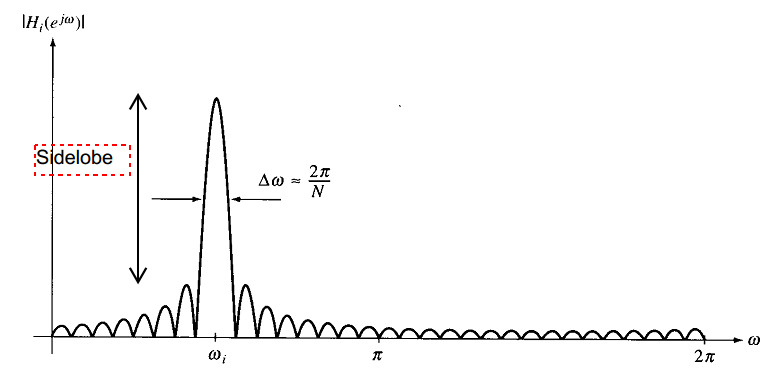
\includegraphics[width=8cm]{./bilder/sidelobe.jpg}
\end{minipage}



 
 
\subsection{Nonparametric Method - Bartlett's Method \hayes{412}}
The idea of Bartlett was to take $K$ non-overlapping sub-sequences (lenght $L$) of the given data. 
A Periodogram (rectangular window) has to be calculated for every sub-sequence and then averaged. $N=K\cdot L$

\begin{tabbing}
power spectrum:  	\=  $\hat{P}_{B}(e^{jw}) = E\left\{\frac{1}{L}  \left|X_L(e^{jw})\right| ^2\right\} =  \frac{1}{N}\sum\limits_{i=0}^{K-1} \left|\sum\limits_{n=0}^{L-1} x(n+iL)e^{-jn\omega}\right| ^2$   \\
Bias: 				\>  $E\left\{ \hat{P}_{B}(e^{jw}) \right\} = \frac{1}{2 \pi}P_x(e^{jw})*W_B(e^{jw})$  \hspace{4cm} \= W $\to$ Bartlet window\\
Resolution: 		\>  $Res\left[\hat{P}_{B}(e^{jw})\right] = \Delta w = 0.89 \cdot K \cdot \frac{2 \pi}{N}$\> Resolution = 3dB BW $(\Delta\omega)_{3dB}$\\
Variance 			\> $Var\left\lbrace\hat{P}_{B}(e^{j\omega})\right\rbrace = \frac{1}{K} Var\left\lbrace \hat{P}_{per}^{(i)}(e^{j\omega}) \right\rbrace \approx \frac{1}{K}P^2_x(e^{j\omega})$\\
\end{tabbing}
So the problem of a bad and inconsistent variance could be eliminated. But the resolution is $K$ times worse.

\subsection{Nonparametric Method - Welch's Method \hayes{415}}
Welch' method is a modification of the Bartlett's method. It uses overlapping of the sub-sequences.
When maintaining $L$ = section length, $K$ = number of sections, $D$ = overlap, the formula 
$\boxed{N=L+D(K-1)}$ can be established. This means, that if $D=L$ there is no overlap and $D=L/2$ means 50\% overlap.

\begin{tabbing}
Power spectrum:  	\=  $\hat{P}_{W}(e^{jw}) =  \frac{1}{KLU}\sum\limits_{i=0}^{K-1} \left|\sum\limits_{n=0}^{L-1} w(n) \cdot x(n+iD)e^{-jn\omega}\right| ^2$   \\
\>						$U = \frac 1L \sum\limits_{n=0}^{L-1}|w(n)|^2$ = equalization factor for the given window\\
Bias: 				\>  $E\left\lbrace \hat{P}_{W}(e^{jw}) \right\rbrace = \frac{1}{2 \pi LU}P_x(e^{jw})*|W(e^{jw})|^2$\\
Resolution: 		\>  Window dependent\\
Variance 			\> $Var\left\lbrace\hat{P}_{W}(e^{j\omega})\right\rbrace \approx \frac{9}{16} \frac{L}{N}P^2_x(e^{j\omega}) = 
\frac{9}{16} Var\left\lbrace\hat{P}_{B}(e^{j\omega})\right\rbrace$ \qquad with Barlett window and 50\% overlap\\
\end{tabbing}


\subsection{Nonparametric Method - Blackman-Tukey \hayes{420}}
The idea of Blackman Tukey is to minimalize the effect of the of the autocorrelation samples with a \em big lag\em, because with finite data record the variance of $\hat{r_x}(k)$ will be large.
This is because these samples just have some few samples that can be averaged.
Therefore, the autocorrelation is weighted with a window (like Hann, Bartlett or Hamming).\\
The window length $M$ has to be much smaller than the length of the autocorrelation $N$: $M  \ll N \Rightarrow M < \frac{1}{5}N$
\begin{tabbing}
Power spectrum:  	\=  $\hat{P}_{BT}(e^{jw}) =  \sum\limits_{k=-M}^{M} \hat{r}_x(k)w(k)e^{-jk\omega} \qquad
						\hat{P}_{BT}(z) =  \sum\limits_{k=-M}^{M} \hat{r}_x(k)w(k)z^{-k}$   \\
Bias: 				\>  $E\left\lbrace \hat{P}_{BT}(e^{jw}) \right\rbrace = \frac{1}{2 \pi}P_x(e^{jw})*W(e^{jw})$  \hspace{2cm} \= W $\to$ choosen window\\
Resolution: 		\>  Winow dependent\\
Variance 			\> $Var\left\lbrace\hat{P}_{BT}(e^{j\omega})\right\rbrace \approx P^2_x(e^{j\omega}) \frac{1}{N} \sum\limits_{k=-M}^{M}w^2(k)$\\
\end{tabbing}

\subsection{Performance Comparison \hayes{424}}
To compare different methods the following criteria can be used:\\
\begin{tabbing}
Variability:   \hspace{1cm}  	\= 
  $\nu=\frac{Var\left\lbrace\hat{P}_{x}(e^{j\omega})\right\rbrace}{E^2\left\lbrace\hat{P}_{x}(e^{j\omega})\right\rbrace}=\frac{\sigma^2}{\mu^2}$ 
  \hspace{1cm} \= it's also called normalized variance (smaller is better)\\
  resolution \> $\Delta \omega$ \> smaller is better\\
  figure of merit					\> $M=\nu\cdot \Delta\omega$ \> smaller is better\\
\end{tabbing}
\begin{tabular}{p{3cm} | p{2cm} p{2.5cm} p{3cm}}
& Variability & Resolution & Figure of Merit\\
& $\nu$	&	$\Delta\omega$	& M \\
\hline\\
Periodogram & 1 & $0.89 \frac{2\pi}{N}$ & $0.89 \frac{2\pi}{N}$\\\\
Bartlett & $\frac{1}{K}$ & $0.89\cdot K \cdot  \frac{2\pi}{N}$ & $0.89 \frac{2\pi}{N}$\\\\
Welch & $\frac{9}{8\cdot K}$ & $1.28 \frac{2\pi}{L}$ & $0.72 \frac{2\pi}{N}$\\\\
Blackman-Tukey (Barlett)& $\frac{2\cdot M}{3\cdot N}$  & $0.64 \frac{2\pi}{M}$ & $0.43 \frac{2\pi}{N}$
\end{tabular}

\subsection{Parametric Method - Minimum Variance Method \hayes{426}}
Power spectrum: $\hat{P}_{MV}(e^{jw}) = \frac{p+1}{e^H R_x^{-1}e} \quad R_x = \text{Autocorrelation Matrix} \quad e=[1,e^{j\omega},\ldots, e^{jp\omega}]^T$

\subsection{Parametric Method - Maximum Entropy Method \hayes{433}}
The idea is to use a infinite autocorrelation. For that we have to interpolate the left (übrigen) samples. 
The maximum entropy method (MEM) use a all pole interpolation.
Because of this, the MEM is really good \textbf{if and only if} a spectrum of an \textbf{all- pole model} is given. The coefficients $a_p(k)$ are calculated using the autoregressive model method in section \ref{sec:autoregressive_model_method}.

\begin{tabbing}
Power spectrum:  	\=  $\hat{P}_{MEM}(e^{jw}) =  \frac{|b(0)|^2}{\left| 1 + \sum\limits_{k=1}^{p} a_p(k)e^{-jk\omega}\right|^2} = 				
						\frac{|b(0)|^2}{\left|e^H a_p\right|^2}$ 
						\hspace{1cm} \= $a_p=[1,a_p(1),\ldots, a_p(k)]^T \quad e=[1,e^{j\omega},\ldots, e^{jp\omega}]^T $ \\
\>						$\epsilon_p = |b(0)|^2 = r_x(0) + \sum\limits_{k=1}^p a_p(k) r_x^*(k)$ \\
\end{tabbing}



\section{Adaptive Filtering}
 
\subsection{Adaptive FIR Filters \hayes{497}}
\begin{minipage}{8cm}
        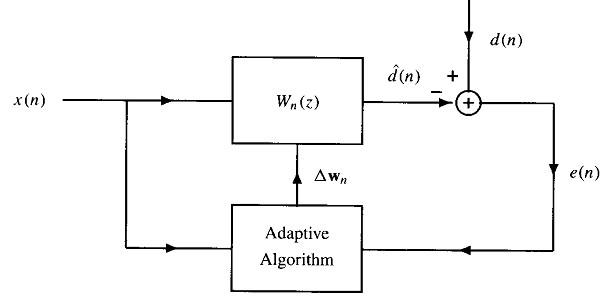
\includegraphics[width=8cm]{./bilder/adaptiveFiltering.jpg}
\end{minipage}
\begin{minipage}{10.5cm}
    \textbf{Goal:} The filter coefficients $w_n$ should be adapted with recursive modification $\Delta w_n$ itself.
    
    \textbf{application area:}
    \begin{liste}
        \item System identification: estimate $H[k], h[n]$ 
        \item Equalize transmission canal  with known sequence: GSM, \ldots
        \item Adaptive noise cancelling (in ear plugs)
        \item Echo cancelling on phone calls
    \end{liste}
\end{minipage}\\
   
The MSE (mean square error) $\xi(w_0, w_1, \ldots, w_n) = E\left(|e(i)|^2\right) = E\left( \left[ d(i) - \sum\limits_{k=0}^{N} w_k x(i-k)\right] ^2 \right)$ should be minimizied. The solution for stationary process is the Wiener-Hopf equations: \\
$$R_x\cdot w = r_{dx}$$
If the process isn't stationary, the filter coefficients have to be updated every step for the optimal result: $w_{n+1}= w_n + \Delta w_n$\\
The adaptive filter should 
\begin{liste}
	\item converge \textbf{to the Wiener-Hopf equations} if the environment is stationary. $\lim\limits_{n\rightarrow\infty} w_n = R_x^{-1}\cdot r_{dx}$
	\item be able to compute the update coefficients $\Delta w_n$, \textbf{without knowledge} of $R_x$ and $r_{dx}$
	\item be able to adapt to the \textbf{changing statistics} and track the solution, if the environment is nonstationary
\end{liste}
\subsubsection{Steepest Descent Adaptive Filter \hayes{499}}
To solve the Wiener-Hopf equations, in every step the autocorrelation matrix has to be inverted and with the crosscorrelation multiplied. 
To reduce this calculations, the coefficient are updated into optimal direction with a small step.
\begin{minipage}{13cm}
$$w_{n+1}=w_n-\mu \cdot  \dfrac{\delta \xi}{\delta w_n} =w_n-\mu \cdot \bigtriangledown\xi(n) \Rightarrow \boxed{ w_{n+1}= w_n+\mu \cdot E\left\lbrace e(n)x^*(n)\right\rbrace}$$ \\
																											$$ \boxed{	w_{n+1}= w_n - \mu \cdot [R_x w_n - r_{dx} ]   }$$ \\
																				%	Stationary solution:	 $ \boxed{	w_{n \to \infty}= w_0 \cdot [R_x w_n - r_{dx} ]^n, n\to \infty   }$
$$ 0<\mu< \frac 2 \lambda_{max}; \lambda_{max} = \text{maximum eigenvalue of autocorrelation matrix } R_x$$
To compute the $E\left\lbrace e(n)x^*(n)\right\rbrace$, a averaging over the last L sample has to be done.  
$$E\left\lbrace e(n)x^*(n)\right\rbrace= \frac{1}{L}\sum\limits_{l=0}^{L-1}e(n-l)x^*(n-l)$$
\end{minipage}
\begin{minipage}{6cm}
        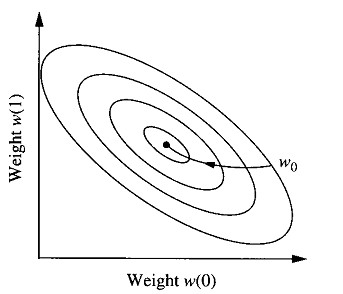
\includegraphics[width=6cm]{../StatDig/bilder/steepestDescent.jpg}
\end{minipage}

 How fast converge the solution/filter: $\displaystyle \tau=\max\{\tau_k\}\approx\frac{1}{\mu \lambda_{min}} $


\clearpage
\subsubsection{LMS Algorithm \hayes{505}}
\begin{minipage}{14cm}

  The LMS algorithm use the same idea as the steepest descent, but just choose the last sample (L=1).\\
  $\boxed{ w_{n+1}=w_n+\mu \cdot e(n) \cdot x^*(n) }$\\
  
  The LMS just converges in the mean, if $\displaystyle 0<\mu< \frac{2}{(p+1)E\left(|x(n)|^2\right)}=\frac{2}{(p+1)r_x(0)}=\frac{2}{(p+1) \cdot \frac{1}{N} \sum\limits_{k=0}^{N-1}|x(n-k)|^2}$.
  The filter coefficients converge to $\hat d(n) = d(n)$ or $e(n) = 0$. 
  That means that filter coefficients always will move, but in the mean they are correct.
\end{minipage}
\begin{minipage}{5cm}
  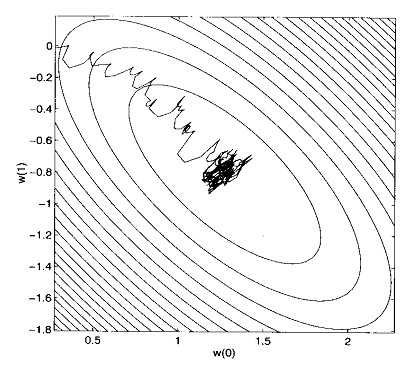
\includegraphics[width=5cm]{../StatDig/bilder/LMS.jpg}
\end{minipage}

\begin{minipage}{9cm}
  \begin{tabbing}
  	Parameters:  \= $p= $ Filter order\\
  	Init:		\> $w_0= 0$\\
  	Computation:
  \end{tabbing}	
      \begin{aufzaehlung}
          \item calculate filter output: $\hat{d}(n) = w_n^T\cdot x(n)$ 
          \item calculate error: $e(n) = d(n) - \hat{d}(n)$
          \item update filter coefficients: $w_{n+1}=w_n+\mu e(n)x^*(n)$  
      \end{aufzaehlung}\vspace{0.05cm}

\end{minipage} 
\begin{minipage}{10cm}
  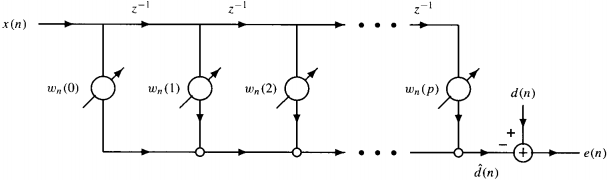
\includegraphics[width=10cm]{../StatDig/bilder/adaptiveFirStructure.png}
\end{minipage}

\subsubsection{Normalized LMS (NLMS) \hayes{514}}
The NLMS is most command used, because it's easy to program, fast to compute and convergence quite fast.\\
The idea is to adapt also the stepsize $\mu(n)=\frac{\beta}{\|x(n)\|^2} \Rightarrow $
$\boxed{w_{n+1}=w_n +\beta \frac{x^*(n)}{\epsilon+\|x(n)\|^2}e(n)}$\\
\begin{liste}
	\item $\|x(n)\|^2$ is the squared sum over $p+1$ samples $\to \sum\limits_{k=0}^{p} | x(n-k) |^2 $, recursively: $\|x(n+1)\|^2 =  \|x(n)\| + |x(n+1)|^2 -|x(n-p)|^2$
 	\item $\epsilon$ is used for small $\|x(n)\|$ (numerical stability)
	\item $\beta$ is a normalized step size with $0 < \beta < 2$
\end{liste}

%Where $\|x(n)\|^2$ is the signal power, $\epsilon$ is used for small $\|x(n)\|$ and is a small positive number and $0<\beta<2$.\\\\
%To reduce the calculation the normalization term $\|x(n)\|$ can also be calculatet recursively:\\ $\|x(n+1)\|^2 =  \|x(n)\| + |x(n+1)|^2 -|x(n-p)|^2$

\subsubsection{Applications - Noise Cancellation \hayes{517}}
\begin{minipage}{9cm}
        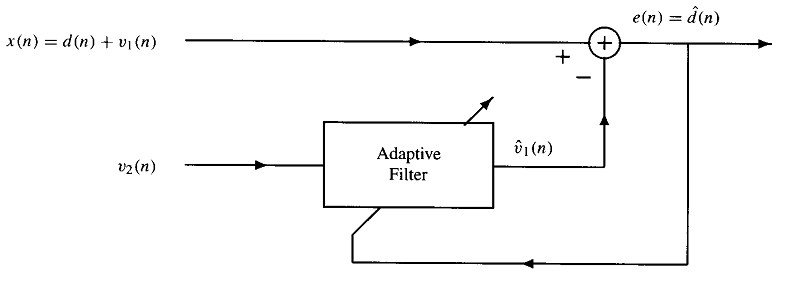
\includegraphics[width=8.5cm]{../StatDig/bilder/adaptiveNoiseCancellation.jpg}\\
        Input signal $x(n)$ with noise (e.g. car noise). 
        The second input measures only the noise (e.g. separate mic). Therefore, $v_1$ and $v_2$ are correlated.
        The filter now guesses the first noise so that the error signal gives the wanted signal $d(n)$.     
\end{minipage}
\hspace{3mm}
\begin{minipage}{9cm}
        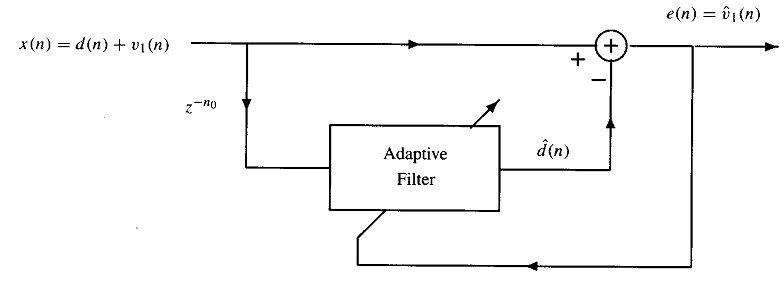
\includegraphics[width=8.5cm]{../StatDig/bilder/NoiseCancellationwithoutRef.jpg}\\
        Input signal $x(n)$ with noise (e.g. car noise). The signal $d(n)$ has to be narrowband and $v_1(n)$ has to be broadband. ($d$ has to be a ``slow''  and $v_1$ has to be a ``fast'' changing signal)
        The filter predicts now $d(n)$ and the error signal is the noise $v_1$.
\end{minipage}

\subsection{Adaptive Recursive Filters (won't be tested) \hayes{534}}
\begin{minipage}{8.4cm}
	Benötigt im Vergleich zum LMS Algorithmus $20M$ nur $2M$ Iterationen bis er konvergiert. RLS nutzt alle vergangene 
	Information zur Berechnung der Korrektur; LMS nutzt nur momentane Information. \\
	$\mathbf{s}(n) = [s(n), s(n-1), \ldots, s(n - N + 1)]^T$ \\
	Forgetting-Faktor ($\mu=1$),
	Initialisierungsfakt. ($\delta = 1)$
\end{minipage}
\begin{minipage}{11cm}
	\begin{aufzaehlung}
	    \item Initialisieren: $n=1; \mathbf{P}(0)=\gamma \cdot \mathbf{I}; \mathbf{\hat{c}}(0)=0$
	    \item Gain Vektor: $ \mathbf{k}(n) = \frac{\mathbf{P}(n-1)\mathbf{s}(n)}{1 + \mathbf{s}^T(n) \mathbf{P}(n-1) \mathbf{s}(n)}$
	    \item Wahrer Schätzfehler: $\eta(n) = r(n) - \mathbf{s}^T(n) \mathbf{\hat{c}}(n-1)$
	    \item Koeffizienten updaten: $\mathbf{\hat{c}}(n) = \mathbf{\hat{c}}(n-1) + \mathbf{k}(n) \eta(n)$
	    \item Fehlerkorrelationsmatrix: \small $\mathbf P(n) = \frac1\mu [ \mathbf P (n-1) - \mathbf k (n) \mathbf u^T (n) \mathbf P(n-1)]$
\normalsize	    \item $n++$ und zurück zu Schritt 2
	\end{aufzaehlung}
\end{minipage}





\end{document}
